\documentclass[12pt,a4paper]{article}

% ============================================================
%  Packages
% ============================================================
\usepackage{fontspec}
\setmainfont{Liberation Serif}
\setsansfont{Liberation Sans}
\setmonofont{Liberation Mono}
\usepackage{polyglossia}
\setdefaultlanguage{russian}
\setotherlanguage{english}
\usepackage{amsmath,amssymb,amsthm,mathtools}
\usepackage[margin=2.5cm]{geometry}
\usepackage[numbers,sort&compress]{natbib}
\usepackage{hyperref}
\usepackage{xcolor}
\usepackage{booktabs}
\usepackage{enumitem}
\usepackage{tikz}
\usetikzlibrary{arrows.meta,positioning,shapes.geometric,decorations.pathmorphing}
\usepackage{float}
\usepackage{microtype}
\tolerance=1500
\emergencystretch=1.5em

% ============================================================
%  Hyperref
% ============================================================
\hypersetup{
  colorlinks=true,
  linkcolor=blue!60!black,
  citecolor=green!50!black,
  urlcolor=blue!60!black,
  pdftitle={Непертурбативная мера спектрального действия},
  pdfauthor={Д. Алфёров, И. Шнюков},
}

% ============================================================
%  Theorem environments (Russian)
% ============================================================
\theoremstyle{plain}
\newtheorem{theorem}{Теорема}[section]
\newtheorem{proposition}[theorem]{Предложение}
\newtheorem{lemma}[theorem]{Лемма}
\newtheorem{corollary}[theorem]{Следствие}
\theoremstyle{definition}
\newtheorem{definition}[theorem]{Определение}
\newtheorem{example}[theorem]{Пример}
\theoremstyle{remark}
\newtheorem{remark}[theorem]{Замечание}

\renewcommand{\proofname}{Доказательство}

% ============================================================
%  Custom commands
% ============================================================
\newcommand{\dd}{\mathrm{d}}
\newcommand{\Tr}{\operatorname{Tr}}
\newcommand{\tr}{\operatorname{tr}}
\newcommand{\HS}{\mathrm{HS}}
\newcommand{\sa}{\mathrm{sa}}
\newcommand{\cF}{\mathcal{F}}
\newcommand{\cB}{\mathcal{B}}
\newcommand{\cP}{\mathcal{P}}
\newcommand{\cG}{\mathcal{G}}
\newcommand{\cO}{\mathcal{O}}
\newcommand{\E}{\mathbb{E}}
\newcommand{\R}{\mathbb{R}}
\newcommand{\N}{\mathbb{N}}
\newcommand{\Lam}{\Lambda}
\newcommand{\half}{\tfrac{1}{2}}
\newcommand{\Id}{\mathrm{Id}}
\newcommand{\Law}{\operatorname{Law}}
\newcommand{\Rep}{\mathrm{Rep}}
\newcommand{\DKL}{D_{\mathrm{KL}}}
\newcommand{\erfi}{\operatorname{erfi}}
\newcommand{\order}{\mathcal{O}}
\DeclareMathOperator{\Stab}{Stab}
\DeclareMathOperator{\rank}{rank}
\DeclareMathOperator{\Herm}{Herm}

% ============================================================
%  Title
% ============================================================
\title{%
  \textbf{Непертурбативная мера спектрального действия:}\\[4pt]
  \textbf{про-торсорная структура и препятствие}\\[2pt]
  \textbf{к каноническим средним}
}
\author{Д.\,Алфёров, И.\,Шнюков\\[4pt]
\small Независимые исследователи\\[2pt]
\small\textit{davidich.alfyorov@gmail.com}}
\date{}

% ============================================================
\begin{document}
\maketitle

\begin{abstract}
В настоящей работе строятся строгие непертурбативные секторные меры
для спектрального действия на операторах Дирака с компактной резольвентой.
В рамках гауссова формализма на пространстве Гильберта--Шмидта
классифицируется препятствие к сборке этих мер в единый функциональный
интеграл.
Наивный евклидов вес $\exp(-\Tr f(D^2/\Lam^2))$ не является
коэрцитивным и приводит к расходящемуся интегралу; для его
регуляризации вводится двусторонняя функциональная гауссова опорная
мера на пространстве самосопряжённых флуктуаций Гильберта--Шмидта,
ковариация которой определяется фоновыми спектральными данными.
Завершённая секторная мера существует, имеет конечную статистическую
сумму и проективно совместима по рангам спектрального усечения.
Различные фоновые секторы, однако, порождают взаимно сингулярные
гауссовы классы (жёсткость Фельдмана--Хайека), что делает
невозможным построение единой вероятностной меры, не зависящей от
фона.  Возникающий глобальный объект есть \emph{про-торсор} локальных
классов мер, оснащённый пучком плотностно-значных наблюдаемых.
Доказывается теорема об отсутствии сечения: относительно любого
выбора опорного веса~$\Phi$ калибровочная группа ограниченных
плотностей действует свободно на нормированных проективных
представителях, исключая дальнейшую каноническую редукцию к
скалярной вероятности без дополнительной структуры.  Классификация
внешних скалярных дополнений требует секторных весов и секторных
терминальных плотностей, подчинённых критерию усечённой
достаточности.  На конечном спектральном ранге всякий разделяющий
канал селектора инъективен и тавтологичен; при аксиоме
нетавтологичности это даёт полный запрет.  Показывается, что все однопетлевые предсказания, извлекаемые из
спектрального действия, универсально сохраняются независимо от
выбора гауссовой опорной меры.
\end{abstract}

\noindent\textit{PACS:} 04.60.--m, 04.62.+v, 11.10.Gh, 02.30.Sa

\tableofcontents
\newpage

% ============================================================
\section{Введение}
\label{sec:intro}
% ============================================================

Принцип спектрального действия, введённый Шамседдином и
Конном~\cite{CC:1996,CC:1997}, постулирует, что бозонная динамика
гравитации, связанной с материей, определяется функционалом
\begin{equation}\label{eq:spectral-action}
  S[D] \;=\; \Tr\, f\!\left(\frac{D^2}{\Lam^2}\right),
\end{equation}
где $D$~--- оператор Дирака почти коммутативной спектральной тройки,
кодирующей Стандартную модель, связанную с евклидовой гравитацией,
$\Lam$~--- масштаб ультрафиолетового обрезания, а
$f\colon [0,\infty)\to [0,\infty)$~--- положительная чётная
пробная функция класса Шварца.  Классическое содержание этого
действия (член Эйнштейна--Гильберта, космологическая постоянная,
потенциал Хиггса и кинетические калибровочные члены) извлекается
из асимптотического разложения~\eqref{eq:spectral-action} по степеням
$\Lam^{-2}$~\cite{CC:1997,CCM:2007,vS:2015}.

Если \emph{классическое} спектральное действие изучено весьма
подробно, то \emph{квантовая} теория~--- функциональный интеграл
по операторам Дирака,
\begin{equation}\label{eq:naive-PI}
  Z \;=\; \int \exp\!\bigl(-S[D]/\hbar\bigr)\,\mathcal{D}[D],
\end{equation}
--- остаётся по большей части формальной.  На конечном спектральном
ранге Барретт и Глейзер~\cite{BarrettGlaser:2016} вычислили интеграл по
случайным некоммутативным геометриям методом Монте-Карло, а в
последующих работах Азарфар--Халхали~\cite{AzarfarKhalkhali:2024} и
Перес-Санчес~\cite{PerezSanchez:2021} исследовали функциональную
ренормализационную группу для усечений типа матричных моделей.  На
однопетлевом уровне ван~Нюланд и ван~Сёйлеком~\cite{vNvS:2022} дали
строгое рассмотрение однопетлевых поправок к спектральному действию.
Однако полная непертурбативная мера $\mathcal{D}[D]$ на
бесконечномерном пространстве операторов Дирака до сих пор не
построена.

Настоящая работа непосредственно обращается к проблеме
непертурбативной меры.  Наши основные результаты:
\begin{enumerate}[leftmargin=2em]
  \item Наивный интеграл~\eqref{eq:naive-PI} \emph{расходится}:
    голый евклидов вес ограничен снизу положительной константой, а
    конфигурационное пространство некомпактно
    (теорема~\ref{thm:divergence}).

  \item Исправленная двусторонняя функциональная гауссова опорная
    мера на самосопряжённом пространстве флуктуаций
    Гильберта--Шмидта $\HS_\sa(H)$ даёт корректно определённую
    \emph{секторную завершённую меру} для каждого фона~$D_0$ с
    компактной резольвентой
    (теорема~\ref{thm:sectorial-existence},
    определение~\ref{def:completed-measure}
    и предложение~\ref{prop:projective}).

  \item Различные фоновые секторы порождают взаимно сингулярные
    гауссовы классы в силу жёсткости Фельдмана--Хайека, даже для
    пертурбативно близких фонов
    (теорема~\ref{thm:feldman-hajek},
    предложение~\ref{prop:fh-close}).  Глобальный объект
    представляет собой \emph{про-торсор} локальных завершённых
    классов мер (теорема~\ref{thm:pro-torsor}).

  \item Карто-независимые средние обычных скалярных наблюдаемых
    \emph{не} определены канонически; лишь сечения дуальной линии
    плотностей канонически спариваются с про-торсором
    (теорема~\ref{thm:scalar-nogo}).

  \item Никакая внутренняя аксиома (симметрия, полуклассическое
    согласование, фоновая ковариантность, данные конечных
    наблюдаемых или хвостовой/асимптотический отбор) не может
    тривиализовать про-торсор: калибровочная группа ограниченных
    плотностей действует свободно на нормированных представителях
    (\emph{главная теорема об отсутствии сечения},
    теорема~\ref{thm:no-section}).

  \item Внешнее скалярное пополнение классифицируется секторными
    весами и секторными терминальными плотностями, подчинёнными
    критерию усечённой достаточности
    (теорема~\ref{thm:external-classification}).
    На конечном спектральном ранге всякий разделяющий
    не зависящий от состояния канал селектора инъективен и, следовательно,
    является тавтологическим перекодированием полного усечения
    (теорема~\ref{thm:tautology}).

  \item Все древесные и однопетлевые предсказания спектральной
    каузальной теории (СКТ) \emph{универсально сохраняются}, независимо
    от выбора гауссовой опорной меры
    (теорема~\ref{thm:one-loop-universality}).
\end{enumerate}

\medskip

\noindent\textbf{Вклад.}\quad
Главный вклад работы состоит из двух утверждений. Позитивное: для каждого фона секторная мера существует, имеет конечную статсумму и совместима по рангам усечения. Негативное: никакой внутренний принцип не склеивает секторные меры в одну; недостающие данные являются внешними и точно классифицированы. Это перекликается с необходимостью граничных данных в каузальной гравитации~\cite{Surya:2019,AJL:2012} и голографических моделях, но здесь данный факт возникает как математическая теорема в рамках спектрального действия, а не как внешнее допущение.

\medskip

\noindent\textbf{Статус.}\quad
Про-торсорная конструкция и главная теорема об отсутствии сечения
\emph{доказаны} безусловно.  Внешняя классификация и теорема о
тавтологичности на конечном ранге \emph{доказаны}.  Полный запрет
(отсутствие допустимой нетавтологической башни селекторов)
\emph{условен}~--- требуется явная аксиома нетавтологичности.
Лоренцево продолжение и связь с факеонным предписанием~\cite{Anselmi:2018} не рассматриваются;
см.\ раздел~\ref{sec:not-shown}.

\medskip

Логика работы следует цепочке, показанной на рис.~\ref{fig:flow}. Мы начинаем с диагноза: наивный интеграл~\eqref{eq:naive-PI} расходится (\S\ref{sec:measure-problem}). Лечение (гауссово пополнение) восстанавливает меру посекторно (\S\ref{sec:gaussian}), но сингулярность Фельдмана--Хайека между секторами порождает про-торсорную структуру (\S\ref{sec:pro-torsor}). Далее мы систематически исключаем все внутренние способы тривиализовать торсор (\S\ref{sec:no-go}), классифицируем оставшиеся внешние выходы (\S\ref{sec:external}) и проверяем, что конструкция содержательна на примере Стандартной модели (\S\ref{sec:SM}) и при сравнении с КДТ и голографией (\S\ref{sec:comparison}). Раздел~\ref{sec:not-shown} подводит черту: что сделано, а что нет.

% ============================================================
%  Рис. 1: Логическая блок-схема
% ============================================================
\begin{figure}[ht]
\centering
\begin{tikzpicture}[
  box/.style={draw, rounded corners=3pt, fill=#1!8, minimum width=5.2cm,
              minimum height=0.75cm, align=center, font=\small},
  box/.default=blue,
  arr/.style={-{Stealth[length=5pt]}, thick, #1},
  arr/.default=black,
  lbl/.style={font=\scriptsize\itshape, fill=white, inner sep=1.5pt},
]
% Узлы
\node[box=red]    (bare)    at (0, 0)    {Голое спектральное действие $e^{-S/\hbar}$};
\node[box=red,    minimum width=4cm] (div)
                            at (0,-1.3)  {\textbf{Расходится} (теор.~\ref{thm:divergence})};
\node[box=blue]   (gauss)   at (0,-2.8)  {Гауссово пополнение $d\gamma_{D_0,\Phi}$};
\node[box=green]  (sect)    at (0,-4.3)  {Секторная мера $\mu_{D_0}^\hbar$ \textbf{существует}};
\node[box=orange] (fh)      at (0,-5.8)  {Фельдман--Хайек: секторы $\perp$ друг другу};
\node[box=violet] (torsor)  at (0,-7.3)  {\textbf{Про-торсор} классов мер};
\node[box=red]    (nosec)   at (-3.5,-8.8) {Теорема об отсутствии сечения};
\node[box=blue]   (ext)     at (3.5,-8.8)  {Классификация внешних селекторов};
\node[box=orange] (taut)    at (0,-10.3) {Конечный ранг: выживают только \textbf{тавтологические}};
% Стрелки
\draw[arr=red!70!black]   (bare)   -- node[lbl,right]{некоэрцитивный} (div);
\draw[arr=blue!70!black]  (div)    -- node[lbl,right]{теор.~\ref{thm:sectorial-existence}} (gauss);
\draw[arr=green!50!black] (gauss)  -- node[lbl,right]{опр.~\ref{def:completed-measure}, пред.~\ref{prop:projective}} (sect);
\draw[arr=orange!70!black](sect)   -- node[lbl,right]{теор.~\ref{thm:feldman-hajek}} (fh);
\draw[arr=violet!70!black](fh)     -- node[lbl,right]{теор.~\ref{thm:pro-torsor}} (torsor);
\draw[arr=red!70!black]   (torsor) -- node[lbl,left,pos=0.4]{теор.~\ref{thm:no-section}} (nosec);
\draw[arr=blue!70!black]  (torsor) -- node[lbl,right,pos=0.4]{теор.~\ref{thm:external-classification}} (ext);
\draw[arr=orange!70!black](nosec)  -- (taut);
\draw[arr=orange!70!black](ext)    -- (taut);
% Примечание об однопетлевой универсальности
\node[draw, dashed, rounded corners, fill=green!5,
      font=\scriptsize, text width=3.8cm, align=center]
      (univ) at (5.8,-4.3) {Однопетлевая универсальность:\\все предсказания СКТ\\сохранены (теор.~\ref{thm:one-loop-universality})};
\draw[-{Stealth[length=4pt]}, dashed, green!50!black] (sect) -- (univ);
\end{tikzpicture}
\caption{Логическая структура работы.  Голый вес спектрального действия
некоэрцитивен и даёт расходящийся интеграл.  Гауссова опорная мера
лечит расходимость посекторно, однако сингулярность Фельдмана--Хайека
между секторами приводит к про-торсорной структуре.  Никакая
внутренняя аксиома не может тривиализовать торсор (главная теорема
об отсутствии сечения); внешние данные классифицированы, но на
конечном ранге допускают лишь тавтологические каналы.
Все однопетлевые предсказания универсально сохранены.}
\label{fig:flow}
\end{figure}

% ============================================================
\section{Спектральное действие и проблема меры}
\label{sec:measure-problem}
% ============================================================

\subsection{Постановка}

Пусть $(H, D_0, \gamma, J)$~--- чётная вещественная спектральная
тройка с компактной резольвентой, где $H$~--- сепарабельное
гильбертово пространство, $D_0$~--- самосопряжённый оператор с
компактной резольвентой, $D_0 e_n = \lambda_n e_n$, $\gamma$~---
градуировка, а $J$~--- вещественная структура.  Собственные значения
упорядочены по неубыванию $|{\lambda_n}|$.

Самосопряжённое пространство флуктуаций Гильберта--Шмидта есть
\begin{equation}\label{eq:HS-space}
  X \;:=\; \HS_\sa(H) \;=\;
  \bigl\{A \in B(H) : A = A^*,\;\Tr(A^2) < \infty\bigr\},
\end{equation}
снабжённое скалярным произведением Гильберта--Шмидта
$\langle A, B\rangle_{\HS} = \Tr(AB)$.

\begin{remark}[Выбор конфигурационного пространства и фиксация калибровки]
\label{rem:HS-choice}
В рамках некоммутативной геометрии физические внутренние
флуктуации $A = \sum a_i[D,b_i]$ являются \emph{ограниченными}
операторами, но не обязательно операторами Гильберта--Шмидта.
Мы работаем на $\HS_\sa(H)$, поскольку это наибольшее пространство,
на котором существуют центрированные гауссовы вероятностные меры с
ядерной ковариацией (см.\ раздел~\ref{sec:gaussian}).
Аргумент расходимости теоремы~\ref{thm:divergence} применим
\emph{a fortiori} к любому подпространству $\HS_\sa(H)$ и
распространяется на любое объемлющее пространство, допускающее
опорную меру, поскольку спектральное действие остаётся ограниченным
$(\dim H)\,f(0)$ на $\HS_\sa(H)$ и сходится к конечному пределу
вдоль любого луча.  На пространствах неограниченных операторов, где
спектральное действие может стать коэрцитивным, проблема меры
принимает иную форму; это выходит за рамки нашего рассмотрения.
Подчеркнём, что внутренние флуктуации почти коммутативных спектральных
троек (калибровочные связности, поля Хиггса) являются ограниченными
операторами, которые в общем случае \emph{не} принадлежат
Гильберту--Шмидту: гладкий оператор умножения на компактном
многообразии ограничен, но не компактен.
Ограничение на $\HS_\sa(H)$ является, таким образом, подлинным
математическим выбором, а не физическим требованием.  Его
обоснование состоит в том, что гауссова опорная мера
(теорема~\ref{thm:sectorial-existence}) требует ядерной ковариации,
которая существует только на $\HS_\sa(H)$ или его подпространствах.
Исключаются \emph{большие} флуктуации, далёкие от любого фона,~---
именно те конфигурации, при которых однопетлевое приближение
нарушается.  Непертурбативная проблема меры для таких конфигураций
требует иных инструментов (например, решёточных или
CDT-дискретизаций~\cite{AJL:2012}) и лежит за пределами настоящей
работы.
Далее, спектральное действие инвариантно относительно унитарного
сопряжения $D \to UDU^*$; конструкция в настоящей работе выполнена
на фиксированном фоновом секторе, где калибровка неявно фиксирована
выбором~$D_0$.
Сингулярность Фельдмана--Хайека из теоремы~\ref{thm:feldman-hajek}
относится к гауссовым классам на различных фоновых картах
$\mathcal{C}(D_0) = D_0 + \HS_\sa(H)$.
Если $D_0' = UD_0U^*$ калибровочно эквивалентен~$D_0$,
естественное сравнение проводится через изоморфизм карт
$J_U(A) = UAU^*$, который является изометрией на~$X$ и удовлетворяет
$(J_U)_*\gamma_{D_0,\Phi} = \gamma_{D_0',\Phi}$,
$(J_U)_*\mu^\hbar_{D_0} = \mu^\hbar_{D_0'}$
(поскольку $C_{D_0',\Phi}(J_U A) = J_U(C_{D_0,\Phi}(A))$ и
$S_{D_0'}(J_U A) = S_{D_0}(A)$ в силу инвариантности следа).
Таким образом, калибровочно эквивалентные фоны \emph{не} порождают
новую сингулярность Фельдмана--Хайека; они дают изоморфные
секторные меры.
Аффинная формула $A \mapsto UAU^* + U[D_0,U^*]$ возникает лишь
при переписывании преобразованного сектора обратно в исходной карте;
для почти-коммутативных фонов Стандартной модели чисто калибровочный
член $U[D_0,U^*]$ есть ограниченный, но generically
\emph{не} гильберта-шмидтов оператор (ненулевой гладкий оператор
умножения на компактном многообразии ограничен, но не компактен),
поэтому данная формула не задаёт действие на~$X$.
Обструкция Камерона--Мартина из приложения~\ref{app:cameron-martin}
относится к таким \emph{сдвигам в фиксированной карте}
(геометрические сдвиги, соответствующие диффеоморфизмам --- внешней
симметрии, отличной от внутренней калибровочной группы в NCG), а не
к межкартному отождествлению~$J_U$.
Соответственно, теорему~\ref{thm:feldman-hajek} следует
интерпретировать как препятствие между калибровочно
\emph{неэквивалентными} фоновыми секторами (различные спектры
= различные калибровочные орбиты), тогда как полная
конструкция на уровне глобального фактора требует явного
калибровочно фиксированного атласа и анализа Фаддеева--Попова;
см.\ раздел~\ref{sec:not-shown}.
\end{remark}

\begin{remark}[Область применимости конструкции]
Важным открытым вопросом является то, \emph{сохраняется} ли
про-торсорное препятствие
(раздел~\ref{sec:pro-torsor}) на более широком конфигурационном
пространстве.  На пространстве, где спектральное действие
коэрцитивно, гауссова опорная мера может оказаться излишней, и
сингулярность Фельдмана--Хайека, обусловленная мультипликативной
структурой гауссовой ковариации, может не возникнуть.
Напротив, негауссовы опорные меры (например, радоновы меры на
пространствах ограниченных операторов) могут породить иной ландшафт
препятствий.  Пока этот вопрос не решён, результаты данной работы
следует понимать как относящиеся к \emph{гауссову завершённому
формализму Гильберта--Шмидта}, а не как безусловные утверждения о
спектральном действии вообще.
\end{remark}

Для фиксированного фона $D_0$ полный оператор Дирака есть
$D = D_0 + A$, где $A \in X$.  Спектральное действие, вычисленное
на флуктуации, имеет вид
\begin{equation}\label{eq:SA-fluctuation}
  S(A) \;:=\; \Tr\, f\!\left(\frac{(D_0+A)^2}{\Lam^2}\right),
\end{equation}
где $f\colon [0,\infty) \to [0,\infty)$~--- положительная чётная
функция класса Шварца.

\subsection{Расходимость наивного интеграла}

Положительность и ограниченность $f$ немедленно ограничивают $S$:

\begin{lemma}\label{lem:bounded}
Для каждого $A \in X$, $S(A) \ge 0$.  На любом конечноранговом
срезе $\Omega_N$ размерности $d_N$,
\begin{equation}
  0 \;\le\; S_N(A) \;\le\; d_N\,f(0).
\end{equation}
В бесконечной размерности ($\dim H = \infty$) полное спектральное
действие $S(A) = \sum_j f(\mu_j^2/\Lam^2)$ конечно для каждого $A$
(так как $f$ шварцева, а $D_0 + A$ имеет собственные значения с
вейлевским ростом), но $S(A) \le S(0) := \sum_j f(\lambda_j^2/\Lam^2)
< \infty$ в общем случае \emph{не} выполняется.
\end{lemma}

\begin{proof}
Поскольку $f \ge 0$, каждое слагаемое $f(\mu_j^2/\Lam^2) \ge 0$,
откуда $S \ge 0$.  На $\Omega_N$ имеется $d_N$ собственных значений,
каждое из которых вносит вклад не более $f(0)$.
\end{proof}

\begin{theorem}[Расходимость наивного интеграла]
\label{thm:divergence}
Пусть $V \subset X$~--- произвольное ненулевое конечномерное
подпространство.  Тогда
\begin{equation}
  \int_V \exp\!\bigl(-S(A)/\hbar\bigr)\,\dd A \;=\; +\infty.
\end{equation}
\end{theorem}

\begin{proof}
Достаточно показать, что $\exp(-S(A)/\hbar)$ ограничено снизу
положительной константой вдоль каждого луча в~$V$, поскольку $V$
содержит неограниченные лучи и полученный ограниченный снизу интеграл
вдоль каждого луча расходится.

Зафиксируем произвольный ненулевой $A_1 \in V$ и рассмотрим луч
$A(t) = tA_1$, $t \in \R$.  Оператор $D(t) := D_0 + tA_1$ имеет
собственные значения $\mu_n(t)$.  Поскольку $A_1 \in \HS_\sa(H)$
компактен, неравенство Вейля даёт
$|\mu_n(t) - \lambda_n| \le t\,\|A_1\|$, откуда
$|\mu_n(t)| \ge |\lambda_n| - |t|\,\|A_1\|$.  Для каждого
фиксированного~$t$ спектральный хвост удовлетворяет
$|\mu_n(t)| \to \infty$ при $n \to \infty$, следовательно,
$f(\mu_n(t)^2/\Lam^2) \to 0$ вдоль хвоста
(ибо $f \ge 0$ и $f(u) \to 0$ при $u \to \infty$).

Действие $S(tA_1) = \sum_n f(\mu_n(t)^2/\Lam^2)$ есть сходящаяся
сумма неотрицательных членов, каждый ограниченный величиной~$f(0)$.
При $|t| \to \infty$ собственные значения $D(t)$ отталкиваются от
начала координат: для любого фиксированного~$R > 0$ лишь конечное число
индексов~$n$ удовлетворяет $|\mu_n(t)| \le R$ при больших~$|t|$
(поскольку $|\lambda_n|$ растёт, а $A_1$ компактен).  Поэтому число
членов, вносящих больше~$\delta$ в сумму, стремится к нулю, и
$S(tA_1) \to c_{A_1}$ для некоторого конечного $c_{A_1} \ge 0$.

Следовательно, $\exp(-S(tA_1)/\hbar) \to \exp(-c_{A_1}/\hbar) > 0$,
и интеграл вдоль луча
$\int_{-\infty}^\infty \exp(-S(tA_1)/\hbar)\,\dd t = +\infty$
(по сравнению с положительной константой на неограниченном
промежутке).  Поскольку $V$ содержит такой луч, $d$-мерный интеграл
по~$V$ расходится.
\end{proof}

\begin{remark}
Теорема~\ref{thm:divergence} показывает, что ни принцип глобального
минимума, ни наивный континуальный интеграл не применимы к
спектральному действию.  Вес $\exp(-S/\hbar)$ по существу постоянен
на бесконечности, а конфигурационное пространство некомпактно.
\emph{Пополнение} экспоненты (посредством опорной меры,
коэрцитивного члена или ограничения области) является
обязательным.
\end{remark}

Гауссово пополнение (раздел~\ref{sec:gaussian}) работает на конечноранговых срезах. Для того чтобы конечноранговые вычисления имели смысл, покажем, что гладко-оконные усечения равномерно сходятся к полному действию вместе с первой и второй производными.

\subsection{Гладко-оконные усечения и сходимость}
\label{subsec:smooth-window}

Для гладкой финитной срезающей функции
$\chi_R \in C_c^\infty(\R)$, $0 \le \chi_R \le 1$,
$\chi_R(\lambda) = 1$ при $|\lambda| \le R$ и
$\mathrm{supp}\,\chi_R \subset \{|\lambda| \le R+1\}$,
определим гладко-оконное усечённое действие
\begin{equation}\label{eq:smooth-window}
  S_R(A) \;:=\; \Tr\bigl(\chi_R(D_0+A)\,f((D_0+A)^2/\Lam^2)\bigr).
\end{equation}
Поскольку $\chi_R(D_0+A)$~--- спектральная функция оператора
$D_0+A$, она коммутирует со всеми ограниченными борелевскими
функциями от $D_0+A$, устраняя несогласованность
проекции/сжатия, свойственную усечениям с замороженным проектором.

\begin{theorem}[Сходимость гладко-оконных усечений]
\label{thm:smooth-convergence}
Допустим выполнение следующих стандартных гипотез спектральной
теории возмущений:
\begin{enumerate}[label=\textup{(A\arabic*)},leftmargin=3em]
  \item\label{A1} Все операторы $D(A) := D_0 + A$ имеют общую
    плотную область определения $\mathrm{Dom}(D_0) \subset H$.
  \item\label{A2} Параметрические производные $\partial_i D$ и
    $\partial_{ij} D$ являются дифференциальными операторами
    первого порядка с равномерно ограниченными матричными элементами:
    $|\langle e_m, \partial_i D\, e_n\rangle| \le C(1+|\lambda_m|)^{1/2}
    (1+|\lambda_n|)^{1/2}$.
  \item\label{A3} Равномерный вейлевский подсчёт:
    $N_A(L) := \#\{n : |\mu_n(A)| \le L\} \le C_K(1+L)^d$ на
    компактных подмножествах параметров $K$.
  \item\label{A4} Шварцевы разделённые разности: первая и вторая
    разделённые разности любой шварцевой функции снова шварцевы на
    $\R^2$ и $\R^3$ соответственно.
\end{enumerate}
Тогда для каждого компактного подмножества параметров $K$
\begin{equation}
  \sup_{A \in K}\,\bigl|\partial_A^\alpha\bigl(S_R(A) - S(A)\bigr)\bigr|
  \;\longrightarrow\; 0
  \qquad\text{при } R \to \infty,
  \quad |\alpha| \le 2.
\end{equation}
Если $f$ имеет шварцево убывание $|f^{(k)}(\lambda)| \le C_k
(1+|\lambda|)^{-M}$ для всех $M$, то скорость сходимости составляет
\begin{equation}\label{eq:convergence-rate}
  \bigl|S_R(A) - S(A)\bigr| \;\le\; C_K\,(1+R)^{d-M}
\end{equation}
для любого $M > 0$, с аналогичными оценками для производных.  Для
экспоненциально убывающих $f(\lambda) \sim e^{-c\lambda}$ скорость
составляет $\order(e^{-cR})$.
\end{theorem}

\begin{proof}[Набросок доказательства]
Запишем $r_R := (1-\chi_R)\cdot h$, где $h(\lambda) :=
f(\lambda^2/\Lam^2)$.  Поскольку $\chi_R = 1$ при $|\lambda| \le R$
и $h$ шварцева, $r_R \to 0$ в шварцевой топологии.  Первая
производная спектрального действия использует формулу
Хеллмана--Фейнмана (кратный операторный интеграл порядка 1),
а вторая производная~--- двойную сумму по разделённым разностям.
При гипотезах \ref{A1}--\ref{A4} оценки матричных элементов и
вейлевский подсчёт обеспечивают равномерную сходимость этих сумм.
Оценка скорости~\eqref{eq:convergence-rate} следует из хвостовой
оценки $|r_R(\lambda)| \le C(1+R)^{-M}$ при $|\lambda| > R$.
Полные подробности приведены в приложении~\ref{app:convergence}.
\end{proof}

\begin{corollary}[Устойчивость седловых точек]
\label{cor:saddle-persistence}
Если $A_* = 0$~--- невырожденная критическая точка $S$ на
калибровочно-фиксированном срезе, то для всех достаточно больших
$R$ функционал $S_R$ имеет единственную близкую критическую точку
$A_R \to A_*$ со сходящимся гессианом.
\end{corollary}

% ============================================================
\section{Исправленный функциональный гауссов формализм и секторное существование}
\label{sec:gaussian}
% ============================================================

Наивный интеграл расходится: вес $e^{-S/\hbar}$ не убывает на бесконечности. Чтобы придать конфигурационному пространству необходимую коэрцитивность, мы вводим объемлющую гауссову опорную меру. Ключевой объект~--- центрированная гауссова мера на $X$ с двусторонней спектральной ковариацией.

\subsection{Двусторонняя функциональная гауссова ковариация}

\begin{definition}\label{def:covariance}
Пусть $\Phi\colon [0,\infty) \to (0,\infty)$~--- положительный
допустимый спектральный вес (например, тепловой
$\Phi(u) = e^{-u}$ или соболевский $\Phi(u) = (1+u)^{-s}$,
$s > 2$).  Определим коэффициенты спектрального убывания
$\phi_n := \Phi(\lambda_n^2/\Lam^2)$ и двусторонний оператор
ковариации
\begin{equation}\label{eq:covariance}
  C_\Phi(A) \;:=\; \sigma^2\, \Phi_0\, A\, \Phi_0,
  \qquad \Phi_0 := \Phi(D_0^2/\Lam^2),
\end{equation}
действующий на $X = \HS_\sa(H)$, где $\sigma^2 > 0$~---
нормировочная константа.
\end{definition}

В собственном базисе $\{E_{mn}\}$ оператора $D_0$ ковариация
действует диагонально на матричных единицах:
$C_\Phi(E_{mn}) = \sigma^2 \phi_m \phi_n\, E_{mn}$.

\begin{theorem}[Критерий ядерности]
\label{thm:trace-class}
Оператор $C_\Phi$ ядерен на $X = \HS_\sa(H)$ тогда и только тогда,
когда
\begin{equation}\label{eq:trace-class-condition}
  \sum_{n=0}^\infty \phi_n \;<\; \infty.
\end{equation}
При выполнении этого условия $\Tr_{\HS}(C_\Phi) = \sigma^2\bigl(\sum_n
\phi_n\bigr)^2$.
\end{theorem}

\begin{proof}
Выберем вещественный ортонормированный базис пространства
$\HS_\sa(H)$, состоящий из диагональных матричных единиц
$F_{nn} := E_{nn}$ и внедиагональных единиц
$(E_{mn} + E_{nm})/\sqrt{2}$ и $i(E_{mn} - E_{nm})/\sqrt{2}$
для $m < n$.  Тогда $C_\Phi(F_{nn}) = \sigma^2 \phi_n^2 F_{nn}$,
что даёт вклад $\sigma^2\phi_n^2$ в след.  Каждая внедиагональная
пара вносит $\sigma^2 \phi_m\phi_n$.  Суммируя:
$\Tr_{\HS}(C_\Phi) = \sigma^2[\sum_n \phi_n^2 + 2\sum_{m<n}
\phi_m\phi_n] = \sigma^2(\sum_n \phi_n)^2$.  Это конечно тогда и
только тогда, когда $\sum_n \phi_n < \infty$.
\end{proof}

\begin{proposition}[Допустимость стандартных спектральных весов]
\label{prop:admissibility}
\hfill
\begin{enumerate}[label=\textup{(\alph*)},leftmargin=2.5em]
  \item Тепловой: $\Phi(u) = e^{-\tau u}$, $\tau > 0$.  Тогда
    $\phi_n = e^{-\tau\lambda_n^2/\Lam^2}$, и $\sum_n \phi_n <
    \infty$ по вейлевской асимптотике $|\lambda_n| \sim n^{1/d}$.
  \item Соболевский: $\Phi(u) = (1+u)^{-s}$, $s > 0$.  Тогда
    $\sum_n \phi_n < \infty$ тогда и только тогда, когда
    $s > d/2$.  Для $d=4$ это требует $s > 2$.
  \item Однопетлевые ядра СКТ: $\Phi(u) \sim c/u$ при
    $u \to \infty$.  Тогда
    $\phi_n \sim c\Lam^2/\lambda_n^2$, откуда
    $\sum_n \phi_n \sim \sum_n n^{-2/d}$, что расходится при
    $d \ge 2$.
    \textbf{Мастер-функция и однопетлевые формфакторы СКТ не
    определяют допустимых ковариаций.}
\end{enumerate}
\end{proposition}

\begin{remark}[Однопетлевые ядра СКТ и опорная мера]
\label{rem:kernels-vs-reference}
Недопустимость однопетлевых ядер СКТ в качестве гауссовых
ковариаций \emph{не} подрывает теорему об однопетлевой
универсальности (теорема~\ref{thm:one-loop-universality}).
Различие состоит между \emph{входом} и \emph{выходом} конструкции:
спектральный вес $\Phi$~--- это \emph{вход}, определяющий опорную
меру, тогда как формфакторы СКТ $h_C, h_R$ являются \emph{выходом}
однопетлевого пертурбативного вычисления вокруг любой допустимой
опорной меры.  Теорема~\ref{thm:one-loop-universality} утверждает,
что этот выход одинаков для всех допустимых $\Phi$ и совпадает со
стандартным результатом стационарной фазы.  Таким образом,
формфакторы СКТ характеризуют универсальное однопетлевое
эффективное действие, а не ковариацию опорной меры.
\end{remark}

\subsection{Теорема о секторном существовании}

\begin{theorem}[Секторная гауссова родительская мера]
\label{thm:sectorial-existence}
Для каждого фиксированного фона $D_0$ с компактной резольвентой и
каждого допустимого веса $\Phi$ с $\sum_n \phi_n < \infty$
существует единственная центрированная гауссова борелева
вероятностная мера
\begin{equation}
  \gamma_{D_0,\Phi}
\end{equation}
на $X = \HS_\sa(H)$ с ковариацией $C_\Phi$.
\end{theorem}

\begin{proof}
Поскольку $C_\Phi$~--- симметричный положительный ядерный оператор
на сепарабельном гильбертовом пространстве $X$, существование и
единственность $\gamma_{D_0,\Phi}$ следуют из стандартной теории
гауссовых мер на сепарабельных гильбертовых пространствах
(см.\ \cite{Bogachev:1998}, глава~3; \cite{Kuo:1975}).
Альтернативно, мера представляет собой произведение одномерных
гауссиан $\mathcal{N}(0, \sigma^2\phi_m\phi_n)$ в собственном базисе,
и произведение сходится по теореме Колмогорова о согласованности,
поскольку произведение дисперсий
$\prod_{m,n}(1 + \sigma^2\phi_m\phi_n)$ сходится при
$\sum_{m,n}\phi_m\phi_n = (\sum_n \phi_n)^2 < \infty$.
\end{proof}

\begin{definition}[Секторная завершённая мера]
\label{def:completed-measure}
\emph{Секторная завершённая мера} для фона $D_0$, спектрального
веса $\Phi$ и параметра петлевого разложения $\hbar > 0$
(введённого как формальный контроль седловой точки; само спектральное
действие $S$ не зависит от $\hbar$, и $\hbar$ входит лишь через
вес $\exp(-S/\hbar)$, играя ту же роль, что и в стандартном
петлевом разложении квантовой теории поля) определяется как
\begin{equation}\label{eq:completed-measure}
  \dd\mu_{D_0}^\hbar(A)
  \;:=\;
  \frac{1}{Z_{D_0}}\,
  \exp\!\left(-\frac{S(A)}{\hbar}\right)
  \dd\gamma_{D_0,\Phi}(A),
\end{equation}
где $Z_{D_0} := \int_X \exp(-S(A)/\hbar)\,\dd\gamma_{D_0,\Phi}(A)$.
\end{definition}

\begin{proposition}[Конечность статистической суммы]
\label{prop:finite-Z}
$0 < Z_{D_0} \le 1$.  Следовательно, $\mu_{D_0}^\hbar$~--- корректно
определённая вероятностная мера на~$X$, абсолютно непрерывная
относительно $\gamma_{D_0,\Phi}$.
\end{proposition}

\begin{proof}
Поскольку $S(A) \ge 0$ для всех $A$, подынтегральное выражение
удовлетворяет $0 < \exp(-S/\hbar) \le 1$.  Отсюда
$0 < Z_{D_0} \le \gamma_{D_0,\Phi}(X) = 1$.
\end{proof}

\subsection{Проективная совместимость}

Пусть $P_N$~--- спектральная проекция $|D_0|$ на первые $N+1$
собственных значений, а $\pi_N(A) := P_N A P_N$~--- отображение
усечения.  Обозначим
$\mu_{D_0,N}^\hbar := (\pi_N)_*\mu_{D_0}^\hbar$ образ меры при
отображении на конечномерное пространство $\Omega_N := P_N X P_N$.

\begin{proposition}[Точная проективная совместимость]
\label{prop:projective}
Для всех $M \ge N$,
$(\pi_{M \to N})_*\,\mu_{D_0,M}^\hbar = \mu_{D_0,N}^\hbar$,
где $\pi_{M \to N}$~--- естественная проекция из $\Omega_M$ в
$\Omega_N$.
\end{proposition}

\begin{proof}
Ковариация $C_\Phi$ диагональна в собственном базисе, поэтому
гауссова опорная мера $\gamma_{D_0,\Phi}$ является произведением
мер.  Усечение $\pi_N$ проецирует на координатное подпространство,
а образ произведения гауссиан на координатном подпространстве
есть соответствующая маргинальная гауссиана.  Поскольку
спектральное действие $S(A)$ зависит от \emph{всех} собственных
значений $D_0 + A$, завершённая мера не является произведением.
Тем не менее, точная проективная совместимость следует из
стандартной дезинтеграции: для пробной функции $\varphi$ на
$\Omega_N$,
\begin{align*}
  \int_{\Omega_N}\varphi\,\dd\mu_{D_0,N}^\hbar
  &= \int_X (\varphi \circ \pi_N)\,\dd\mu_{D_0}^\hbar
  = \frac{1}{Z}\int_X (\varphi\circ\pi_N)\,e^{-S/\hbar}\,\dd\gamma \\
  &= \frac{1}{Z}\int_{\Omega_M}
    \left(\int_{\pi_{M\to N}^{-1}(x)}
      (\varphi\circ\pi_{M\to N})(y)\,e^{-S(y)/\hbar}
    \,\dd\gamma^x(y)\right)\dd\gamma_M(x),
\end{align*}
что даёт одинаковый результат при проекции сначала на $\Omega_M$
и затем на $\Omega_N$ или непосредственно на $\Omega_N$.
\end{proof}

\subsection{Однопетлевая универсальность}
\label{subsec:one-loop}

\begin{theorem}[Однопетлевая универсальность средних]
\label{thm:one-loop-universality}
Пусть $\Phi$ и $\Psi$~--- два допустимых спектральных веса, оба с
$\sum_n \phi_n < \infty$ и $\sum_n \psi_n < \infty$.
Предположим, что фон $A_* = 0$ является невырожденной критической
точкой физического действия $S_N$ (т.\,е.\ гессиан $H_{*,N} :=
\nabla^2 S_N(0)$ положительно определён на~$\Omega_N$).
Тогда для любой $O \in C^3_b(\Omega_N)$,
\begin{equation}\label{eq:one-loop-univ}
  \langle O \rangle_\Phi
  \;=\; O(0)
  + \frac{\hbar}{2}\sum_i \frac{\partial^2 O}{\partial \xi_i^2}(0)\,
    (H_*^{-1})_{ii}
  + \order(\hbar^2)
  \;=\; \langle O \rangle_\Psi,
\end{equation}
где $\xi_i$~--- координаты главных осей на $\Omega_N$,
диагонализирующие $H_{*,N}$, а
$H_* = \nabla^2 S(0)|_{\mathrm{phys}}$~--- гессиан на
физическом срезе в точке фона.  Опорная мера $\Phi$ входит в
средние значения лишь в порядке $\order(\hbar^2)$.
\end{theorem}

\begin{proof}
Поскольку $O$ зависит лишь от конечноранговой проекции
$\pi_N(A) \in \Omega_N$, мы работаем на $\Omega_N$
(размерности $d_N$) на всём протяжении; интеграл по
комплементарным (высоким) модам тождественно факторизуется в
числителе и знаменателе отношения
$\langle O\rangle_\Phi = N/Z$ и сокращается.

На \emph{конечномерном} срезе $\Omega_N$ запишем завершённую меру
как
$\dd\mu_N^\hbar(x) \propto \exp\bigl(-S_N(x)/\hbar
- x^T C_{\Phi,N}^{-1} x/2\bigr)\,\dd x$,
где $S_N$~--- усечённое действие, а $C_{\Phi,N}$~--- маргинальная
ковариация размера $d_N \times d_N$.  Эффективная точность на
$\Omega_N$ есть
\[
  Q_{\hbar,N} \;=\; \frac{H_{*,N}}{\hbar} + C_{\Phi,N}^{-1},
\]
где $H_{*,N} = \nabla^2 S_N(0)$.  Поскольку $\Omega_N$
конечномерно, обе матрицы $H_{*,N}$ и $C_{\Phi,N}^{-1}$ имеют
размер $d_N \times d_N$, и ряд Неймана
\[
  Q_{\hbar,N}^{-1}
  = \hbar\,H_{*,N}^{-1}
  - \hbar^2\,H_{*,N}^{-1}C_{\Phi,N}^{-1}H_{*,N}^{-1}
  + \order(\hbar^3)
\]
сходится при достаточно малых $\hbar$ (а именно при
$\hbar < \|H_{*,N}^{-1}\|^{-1}\|C_{\Phi,N}^{-1}\|^{-1}$, что
положительно, так как обе матрицы конечномерны и положительно
определены).  Ведущая ковариация $\hbar\,H_{*,N}^{-1}$ не зависит
от~$\Phi$.

Стандартная конечномерная формула Лапласа для отношения
$\langle O\rangle = N/Z$ тогда даёт
\[
  \langle O\rangle_\Phi
  = O(0) + \frac{\hbar}{2}\,\Tr\bigl(O''(0)\,H_{*,N}^{-1}\bigr)
  + \order(\hbar^2),
\]
что зависит лишь от физического гессиана $H_{*,N}$, но не
от~$C_{\Phi,N}$.  $\Phi$-зависимая поправка входит в порядке
$\order(\hbar^2)$ через подведущий член
$\hbar^2 H_{*,N}^{-1}C_{\Phi,N}^{-1}H_{*,N}^{-1}$.

\emph{Факторизация высоких мод.}
Обозначим $\Omega_N^\perp$ комплементарное спектральное подпространство.
В спектральном собственном базисе оператора~$D_0$ физический гессиан
$H_* = \nabla^2 S(0)$ действует диагонально на матричных единицах
$E_{mn}$, поэтому перекрёстный блок $H_{*,\mathrm{low\text{-}high}} = 0$
в квадратичном порядке.
Запишем $S(x,y) = S_N(x) + S_\perp(y) + S_{\mathrm{mix}}(x,y)$,
где $S_{\mathrm{mix}} = O(|x|\,|y|^2) + O(|x|^2\,|y|)$ начинается с
кубического порядка.  Гауссова опорная мера $\gamma_\Phi$ обладает
структурой произведения: $\gamma_\Phi = \gamma_{\Phi,N}\otimes\gamma_{\Phi,\perp}$.
Поэтому маргинал меры
$e^{-S/\hbar}\,d\gamma_\Phi$ на $\Omega_N$ равен
\[
  \Bigl[\int_{\Omega_N^\perp} e^{-S_\perp(y)/\hbar
  - S_{\mathrm{mix}}(x,y)/\hbar}\,
  \dd\gamma_{\Phi,\perp}(y)\Bigr]\,
  e^{-S_N(x)/\hbar}\,\dd\gamma_{\Phi,N}(x).
\]
В квадратичном порядке ($\hbar \to 0$) член $S_{\mathrm{mix}}$ подведущий,
выражение в скобках становится независимым от $x$ и сокращается в отношении
$\langle O\rangle = N/Z$
для любой~$O$ с носителем на~$\Omega_N$.
$\Phi$-зависимость выражения в скобках является общим множителем
в~$N$ и~$Z$; его первая $x$-зависимая поправка входит в порядке
$O(\hbar^2)$ через кубические вершины действия~$S$.
\end{proof}

\begin{remark}[Область универсальности: средние и статистическая сумма]
\label{rem:univ-scope}
Теорема~\ref{thm:one-loop-universality} устанавливает
$\Phi$-независимость для \emph{нормированных средних}
$\langle O\rangle = N/Z$, где $\Phi$-зависимые множители
сокращаются в отношении.  Сама \emph{статистическая сумма}~$Z$
зависит от $\Phi$ даже в ведущем порядке (через нормировочные
константы $\gamma_\Phi$).  \emph{Однопетлевое эффективное действие}
$\Gamma^{(1)} = \half\Tr\log H_*$ в литературе по СКТ определяется
через $\zeta$-функциональную регуляризацию физического гессиана
$H_*$ (см.~\cite{Alfyorov:2026ff}), которая является внутренним
спектральным инвариантом $H_*$ и по построению не зависит
от~$\Phi$.  Любая однопетлевая величина, извлекаемая из
$\Gamma^{(1)}$ (формфакторы, спектральные коэффициенты, полюса
пропагатора), поэтому $\Phi$-независима.
См.\ приложение~\ref{app:alpha} для конкретных числовых значений.
\end{remark}

\begin{remark}[Статус за пределами одной петли]
\label{rem:beyond-one-loop}
Зависимость от $\Phi$ в порядке $\order(\hbar^2)$ означает, что
двухпетлевые и высшие поправки \emph{не} универсальны: они несут
отпечаток опорной меры.  Это допускает три интерпретации:
(i)~спектральное действие~--- эффективная теория, применимая лишь
на однопетлевом уровне, а неоднозначность опорной меры поглощает
неизвестную ультрафиолетовую физику;
(ii)~некий физический принцип (пока не найденный) выделяет
предпочтительное $\Phi$, восстанавливая предсказательность на
двухпетлевом уровне;
(iii)~плотностно-значный формализм про-торсора является правильной
основой, и двухпетлевые <<предсказания>> должны формулироваться как
сечения линии плотностей, а не как скалярные числа.
Настоящая работа не разрешает выбор между (i)--(iii); она лишь
устанавливает формализм, в котором вопрос ставится точно.
Отметим, что интерпретация~(i) является спектрально-геометрическим
аналогом хорошо известной ситуации: общая теория относительности,
рассматриваемая как эффективная полевая теория~\cite{Donoghue:1994},
предсказательна на однопетлевом уровне, но приобретает
схемозависимые поправки на двухпетлевом, параметризующие
неизвестную ультрафиолетовую физику.  Зависимость от $\Phi$ в порядке
$\order(\hbar^2)$ играет ту же роль, что и зависимость от схемы
ренормировки в гравитационной ЭТП, и столь же не патологична.
Отметим, что аналогия со схемной зависимостью носит эвристический
характер: в стандартной ЭТП физические наблюдаемые остаются
схемонезависимыми на любом конечном петлевом порядке при включении
всех контрчленов, тогда как зависимость от опорной меры отражает
неполноту непертурбативного определения, а не обычную
ренормировочную неоднозначность.
\end{remark}

\begin{remark}\label{rem:universality-consequence}
Теорема~\ref{thm:one-loop-universality} физически существенна: она
гарантирует, что однопетлевые результаты спектральной каузальной теории,
представленные в~\cite{Alfyorov:2026ff,Alfyorov:2026ss,Alfyorov:2026ct},~---
коэффициент при квадрате Вейля
$\alpha_C = 13/120$~\cite{Alfyorov:2026ff}, полюс призрака и
масса факеона~\cite{AlfyorovShnyukov:2026ns}, а также ограничения
на параметризованные пост-ньютоновские
параметры~\cite{Alfyorov:2026ss}~--- \emph{не зависят} от выбора
гауссовой опорной меры.
(Отметим, что работы~\cite{Alfyorov:2026ff,Alfyorov:2026ss,%
AlfyorovShnyukov:2026ns} являются препринтами, находящимися на
рецензировании; цитируемые однопетлевые результаты самодостаточны
и независимо проверяемы по содержащимся в них выводам.)
\end{remark}

\subsection{Конкретный пример: двухмодовая матричная модель}
\label{subsec:example}

Для наглядности рассмотрим простейший нетривиальный случай:
двумерное гильбертово пространство $H = \mathbb{C}^2$ с фоном
$D_0 = \mathrm{diag}(\lambda_1, \lambda_2)$,
$\lambda_1 \ne \lambda_2$.  Спектральное действие есть
\begin{equation}
  S(A) = f\!\left(\frac{(\lambda_1+a_{11})^2}{\Lam^2}\right)
       + f\!\left(\frac{(\lambda_2+a_{22})^2}{\Lam^2}\right)
\end{equation}
где для простоты ограничиваемся диагональными флуктуациями
$A = \mathrm{diag}(a_{11}, a_{22})$ (внедиагональные элементы
перемешивают собственные значения нелинейно, но не влияют на
аргумент расходимости).

\begin{example}[Двухмодовый завершённый интеграл]
\label{ex:two-mode}
Голый интеграл $\int_{\R^2} e^{-S(a)/\hbar}\,\dd a$ расходится по
теореме~\ref{thm:divergence}: вдоль $a_{11} \to \infty$ при
$a_{22} = 0$ имеем $S \to f(\lambda_2^2/\Lam^2) > 0$~--- константа,
так что подынтегральное выражение ограничено снизу.

С гауссовой опорной мерой $\dd\gamma(a) \propto
\exp(-a_{11}^2/(2\sigma^2\phi_1^2) - a_{22}^2/(2\sigma^2\phi_2^2))\,
\dd a$ завершённый интеграл равен
\begin{equation}
  Z = \int_{\R^2} e^{-S(a)/\hbar}\,\dd\gamma(a)
  \;\le\; 1,
\end{equation}
что конечно и положительно.  Однопетлевое приближение даёт
\[
  Z \approx e^{-S_*/\hbar}\,\frac{2\pi\hbar}{\sqrt{H_{11}H_{22}}},
\]
не зависящее от $\sigma$ и~$\phi_j$.

Рассмотрим теперь второй фон $D_0' = \mathrm{diag}(\lambda_1',
\lambda_2')$ с $\lambda_j' \ne \lambda_j$.  Гауссовы опорные
меры $\gamma$ и $\gamma'$ имеют различные ковариации
($\phi_j \ne \phi_j'$), но в двух измерениях обе являются
невырожденными гауссианами на $\R^2$, а значит, \emph{эквивалентны}
(не сингулярны).  Это иллюстрирует два ключевых момента:
(1)~гауссово пополнение устраняет расходимость на любом ранге;
(2)~на \emph{конечном ранге} сингулярность Фельдмана--Хайека не
возникает~--- различные фоны дают эквивалентные (не сингулярные)
меры.  Про-торсорная структура~--- явление подлинно бесконечномерное
(раздел~\ref{sec:pro-torsor}).
\end{example}

\begin{figure}[ht]
\centering
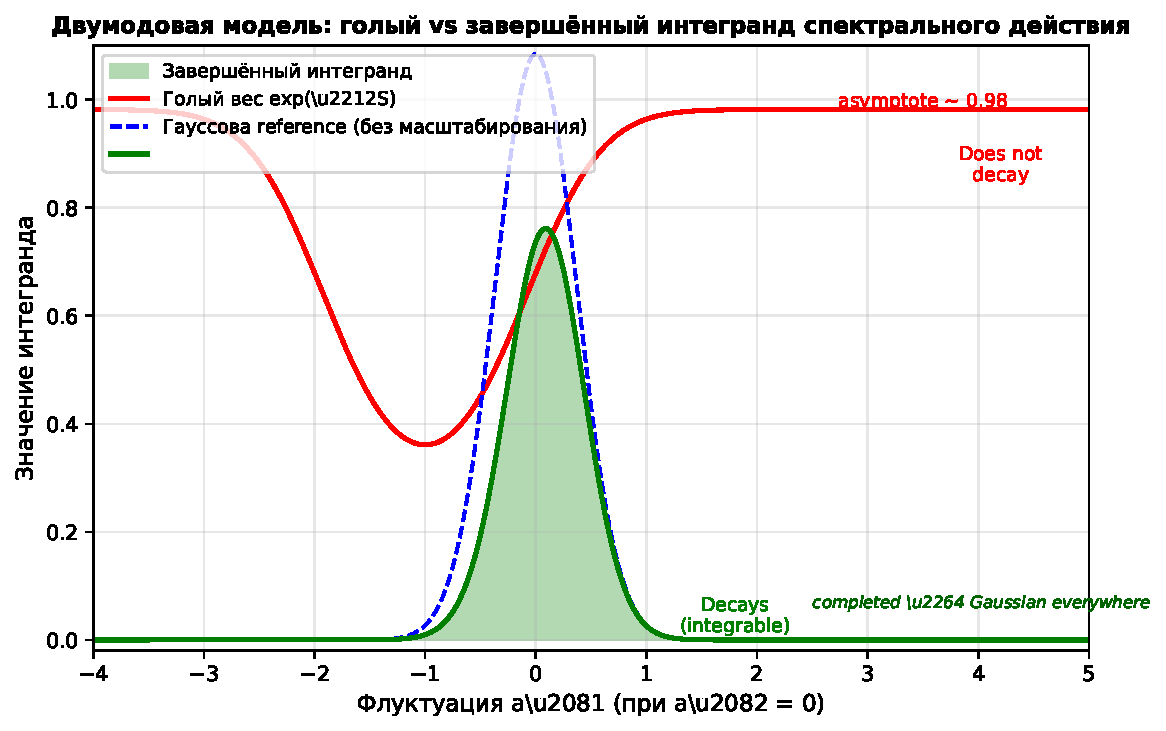
\includegraphics[width=0.82\textwidth]{figures/fig_nonpert_2mode_ru.pdf}
\caption{Двухмодовая матричная модель ($H = \mathbb{C}^2$,
$D_0 = \mathrm{diag}(1,2)$, $f(u) = e^{-u}$, $\Lam = 1$).
Красный: голое подынтегральное выражение $e^{-S(a_1,0)/\hbar}$ не
убывает при $|a_1| \to \infty$ (стремится к
$e^{-f(\lambda_2^2)} \approx 0{,}98$), что делает наивный интеграл
расходящимся (теорема~\ref{thm:divergence}).
Зелёный: завершённое подынтегральное выражение, перевзвешенное
гауссовой опорной мерой $d\gamma$ с ковариацией
$\sigma^2\phi_1^2 \approx 0{,}135$ ($\hbar = \sigma = 1$), быстро
убывает и даёт конечную статистическую сумму $Z \approx 0{,}67$.
Синий пунктир: плотность гауссовой опорной меры (без масштабирования).
Поскольку $S \ge 0$, завершённый интегранд ограничен сверху гауссовой
плотностью всюду: $e^{-S}\,d\gamma \le d\gamma$.
Интегралы вычислены квадратурой \texttt{mpmath} с рабочей точностью
100 знаков и абсолютной погрешностью~$10^{-50}$.}
\label{fig:2mode}
\end{figure}

% ============================================================
\section{Про-торсорная структура и плотностно-значные наблюдаемые}
\label{sec:pro-torsor}
% ============================================================

Итак, секторные меры существуют и проективно совместимы. Естественный вопрос: можно ли склеить их в единый интеграл? Ответ отрицателен, и причина глубока: гауссовы классы различных фонов взаимно сингулярны.

\subsection{Сингулярность Фельдмана--Хайека}

\begin{theorem}[Жёсткость Фельдмана--Хайека для спектральных ковариаций]
\label{thm:feldman-hajek}
Пусть $D_0$ и $D_0'$~--- два фона с компактной резольвентой,
\emph{имеющие общий собственный базис}, с собственными значениями
$\{\lambda_n\}$ и $\{\lambda_n'\}$, и пусть $\gamma_{D_0,\Phi}$ и
$\gamma_{D_0',\Phi}$~--- соответствующие центрированные гауссовы
меры на $X = \HS_\sa(H)$ с одним и тем же спектральным
весом~$\Phi$.  Тогда $\gamma_{D_0,\Phi} \perp \gamma_{D_0',\Phi}$,
если только $\phi_n = \phi_n'$ для всех~$n$.  В частности, любое
нетривиальное изменение фоновых собственных значений (при
фиксированном собственном базисе) порождает взаимно сингулярную
гауссову опорную меру.
\end{theorem}

\begin{proof}
По теореме Фельдмана--Хайека~\cite{Feldman:1958,Hajek:1958,Bogachev:1998}
две центрированные гауссовы меры на сепарабельном гильбертовом
пространстве либо эквивалентны, либо взаимно сингулярны; эквивалентность
имеет место тогда и только тогда, когда
$C_\Phi^{-1/2} C_{\Phi'} C_\Phi^{-1/2} - I$ является
оператором Гильберта--Шмидта.

В собственном базисе оператора $D_0$
(общий случай вытекает из абстрактного критерия)
собственные значения оператора
$C_\Phi^{-1/2} C_{\Phi'} C_\Phi^{-1/2}$ на матричной единице $E_{mn}$
равны $r_m r_n$, где $r_n := \phi_n'/\phi_n$.  Условие Гильберта--Шмидта
принимает вид $\sum_{m,n}(r_m r_n - 1)^2 < \infty$.  Обозначая
$s_k := r_k - 1$:
\[
  r_m r_n - 1 = s_m + s_n + s_m s_n.
\]
Для любого фиксированного $m$ с $s_m \ne 0$ покажем, что сумма по~$n$
расходится.  Возникают два случая.

\emph{Случай~1: $r_n \to 1$ (т.\,е. $s_n \to 0$).}  Это имеет место,
когда возмущение собственных значений достаточно мало, так что
$\phi_n'/\phi_n \to 1$ вдоль спектрального хвоста.
Тогда для всех достаточно больших~$n$ выполняется
$|s_n| < |s_m|/2$, откуда $(r_m r_n - 1)^2 = (s_m(1+s_n)+s_n)^2
\ge (|s_m|/2)^2 = s_m^2/4 > 0$.

\emph{Случай~2: $r_n \not\to 1$.}  Если $r_n \to c \ne 1$
(включая $c = 0$ или $c = +\infty$, что происходит при росте
$\lambda_n' - \lambda_n$), то $r_m r_n - 1 \to r_m c - 1 \ne 0$
для бесконечно многих $n$, и каждое такое слагаемое вносит
положительную константу.

В обоих случаях хвост суммы по~$n$ содержит бесконечно много
слагаемых, ограниченных снизу положительной константой, что даёт
\[
  \sum_{n=0}^\infty (r_m r_n - 1)^2 \;=\; +\infty.
\]
Следовательно, двойная сумма конечна лишь при $s_m = 0$ для
\emph{каждого} $m$, т.\,е. $r_m = 1$ и $\phi_m = \phi_m'$
для всех~$m$.
\end{proof}

\begin{remark}[Общий случай]
\label{rem:fh-general}
Теорема~\ref{thm:feldman-hajek} сформулирована для фонов с общим
собственным базисом.  Когда $D_0$ и $D_0'$ имеют различные собственные
базисы, операторы ковариации $C_\Phi$ и $C_{\Phi'}$ не
диагонализуются одновременно, и критерий Фельдмана--Хайека
включает полный оператор
$C_\Phi^{-1/2}C_{\Phi'}C_\Phi^{-1/2} - I$, а не произведение
скалярных отношений.  Мы предполагаем, что сингулярность
сохраняется и в этом случае, поскольку любое $\varepsilon$-возмущение
спектра меняет спектральные веса $\phi_n$; полное доказательство
для недиагонального оператора оставлено для будущей работы.
\end{remark}

\begin{proposition}[Универсальная сингулярность для пертурбативно
близких фонов]
\label{prop:fh-close}
Пусть $D_0$ и $D_0'$~--- два фона с компактной резольвентой,
\emph{имеющие общий собственный базис}, для которых
$\phi_k \ne \phi_k'$ хотя бы при одном индексе~$k$.
Тогда $\gamma_{D_0,\Phi} \perp \gamma_{D_0',\Phi}$.
В частности, если $D_0' = D_0 + \varepsilon K$ при $\varepsilon > 0$
и $K$~--- любое ненулевое самосопряжённое возмущение, изменяющее
хотя бы одно собственное значение оператора $D_0$, то меры
взаимно сингулярны~--- даже для сколь угодно малого $\varepsilon$
и даже для $K$ конечного ранга.
\end{proposition}

\begin{proof}
Если $\phi_k \ne \phi_k'$, положим $s_k = r_k - 1 \ne 0$.  Тогда
$\sum_n (r_k r_n - 1)^2 \ge \sum_n s_k^2 = +\infty$
(бесконечно много слагаемых), и сумма Фельдмана--Хайека
расходится; по теореме~\ref{thm:feldman-hajek} следует
сингулярность.
\end{proof}

\begin{remark}\label{rem:fh-sharpness}
Сила предложения~\ref{prop:fh-close} заслуживает особого
внимания.  В отличие от стандартной теории гауссовых мер
на $\ell^2$ (где изменение дисперсии одной координаты
сохраняет эквивалентность), \emph{мультипликативная структура}
спектральной ковариации
$C_\Phi(E_{mn}) = \sigma^2\phi_m\phi_n$ означает, что
изменение единственного коэффициента спектрального
убывания $\phi_k$ влечёт изменение собственного значения
ковариации для \emph{каждой} матричной единицы $E_{kn}$,
$n = 0,1,2,\ldots$~--- бесконечно многих собственных значений.
Именно поэтому даже возмущение ранга 1 оператора $D_0$
порождает взаимную сингулярность на бесконечномерном
пространстве $\HS_\sa(H)$.

На \emph{конечном} спектральном ранге $N$ (пример~\ref{ex:two-mode})
конфигурационное пространство $\Omega_N$ конечномерно, и все
невырожденные гауссианы эквивалентны~--- дихотомия
Фельдмана--Хайека не применяется.  Сингулярность есть
подлинно бесконечномерное явление, обусловленное
мультипликативной структурой гауссианов на операторном
пространстве.
\end{remark}

\begin{remark}[Зависимость от анзаца ковариации]
Универсальная сингулярность предложения~\ref{prop:fh-close} зависит от
мультипликативной структуры
$C_\Phi(E_{mn}) = \sigma^2\phi_m\phi_n$
двусторонней ковариации.  Иной анзац ковариации (например,
диагональный в энергетическом базисе с независимыми
дисперсиями или антикоммутаторная форма
$\Phi_0 A + A\Phi_0$) мог бы дать иную картину сингулярности;
в частности, ковариации без мультипликативной структуры не
обязаны усиливать единичное спектральное изменение до
бесконечного числа координат.  Физическое содержание
предложения~\ref{prop:fh-close}, таким образом, привязано
к двусторонней структуре~\eqref{eq:covariance}, являющейся
естественным спектрально-эквивариантным, но не единственным
выбором.
\end{remark}

\subsection{Про-торсорная конструкция}

Поскольку пополненные меры
$\{\mu_{D_0}^\hbar\}_{D_0 \in \mathcal{B}}$ для различных
фонов принадлежат взаимно сингулярным классам мер, их нельзя
собрать в единую вероятностную меру.  Вместо этого они
образуют \emph{про-торсор}.

Обозначим через $\mathcal{B}^{\mathrm{reg}}$ множество регулярных
фонов с компактной резольвентой (допускающих локальные карты
с гладкими функциями перехода), и пусть $\{U_a\}_{a \in \mathcal{A}}$~---
регулярный атлас.  Для каждой карты $U_a$ и спектрального
ранга $N$ пополненная мера конечного ранга $\mu_{a,N}^\hbar$
есть вероятностная мера на конечномерном пространстве
$\Omega_{a,N}$.

На пересечениях $U_a \cap U_b$ меры $\mu_{a,N}^\hbar$ и
$(F_{ab,N})_*\mu_{a,N}^\hbar$ взаимно абсолютно непрерывны
(на конечном ранге гауссианы с различными средними/ковариациями
эквивалентны, а не сингулярны).  Производная Радона--Никодима
\begin{equation}
  g_{ab,N} \;:=\; \frac{\dd(F_{ab,N})_*\mu_{a,N}^\hbar}
    {\dd\mu_{b,N}^\hbar}
\end{equation}
является строго положительной измеримой функцией,
удовлетворяющей коцикловому условию Чеха
\begin{equation}\label{eq:cocycle}
  g_{ac,N} = g_{bc,N}\,g_{ab,N}
  \qquad\text{на тройных пересечениях}.
\end{equation}

\begin{theorem}[Существование про-торсора]
\label{thm:pro-torsor}
Коциклы перехода $\{g_{ab,N}\}$ определяют проективную систему
$\mathcal{T}_\bullet = \{\mathcal{T}_N\}_{N \ge 0}$
$\R_{>0}$-торсоров на регулярном допустимом атласе.  Отображения
усечения $\pi_{M \to N}$ переплетают торсоры на различных
уровнях, превращая $\mathcal{T}_\bullet$ в про-торсор.
\end{theorem}

\begin{proof}
Коцикловое условие~\eqref{eq:cocycle} проверяется по цепному
правилу для производных Радона--Никодима.  При каждом фиксированном
$N$ это определяет $\R_{>0}$-торсор по стандартной теории пучков.
Переплетение следует из проективной совместимости
(предложение~\ref{prop:projective}): прямой образ при
$\pi_{M \to N}$ переводит коцикл уровня $M$ в коцикл
уровня $N$.
\end{proof}

\begin{remark}[Конечный ранг и проективный предел]
\label{rem:finite-vs-limit}
Важно отметить, где живёт торсорная структура и где
проявляется препятствие.  На каждом фиксированном конечном
ранге $N$ меры на пересечениях взаимно абсолютно непрерывны
(конечномерные гауссианы с различными параметрами
эквивалентны, а не сингулярны), поэтому торсор $\mathcal{T}_N$
существует и даже гладко тривиализуем аргументом разбиения
единицы.  Препятствие Фельдмана--Хайека
(теорема~\ref{thm:feldman-hajek}) проявляется лишь
в \emph{проективном пределе} $N \to \infty$, где различные
фоновые секторы порождают взаимно сингулярные объемлющие
меры.  Про-торсор $\mathcal{T}_\bullet$ кодирует этот
переход: каждый конечный уровень тривиализуем, но вся башня~---
нет, поскольку невозможно выбрать проективно согласованную
тривиализацию одновременно на всех уровнях (это содержание
главной теоремы об отсутствии сечения, теорема~\ref{thm:no-section}).
\end{remark}

\subsection{Запрет на скалярные средние}

\begin{theorem}[Запрет на скалярные средние]
\label{thm:scalar-nogo}
Следующие условия эквивалентны:
\begin{enumerate}[label=\textup{(\roman*)},leftmargin=2.5em]
  \item Для каждой ограниченной измеримой скалярной наблюдаемой $O$
    на $\Omega_N$ интеграл $\int O\,\dd\nu_{a,N}$ не зависит от карты
    при любом выборе нормированного представителя $\nu_{a,N}$
    в торсоре.
  \item На каждом пересечении $\nu_{b,N} = (F_{ab,N})_*\nu_{a,N}$.
  \item Все коциклы перехода тривиальны: $g_{ab,N} = 1$.
\end{enumerate}
Нетривиальный про-торсор не определяет канонически средних
обычных скалярных наблюдаемых.
\end{theorem}

\begin{proof}
(i)$\Rightarrow$(iii): Применяя~(i) к индикаторным функциям, получаем:
если $\int 1_U\,\dd\nu_{a,N} = \int 1_U\,g_{ab,N}\,\dd\nu_{a,N}$ для
всех измеримых $U$, то $g_{ab,N} = 1$ п.\,в.
(iii)$\Rightarrow$(ii)$\Rightarrow$(i) очевидно.
\end{proof}

\begin{figure}[ht]
\centering
\begin{tikzpicture}[
  sector/.style={draw, thick, rounded corners=8pt, fill=#1!6,
                 minimum width=3.0cm, minimum height=2.8cm},
  sector/.default=blue,
  inner/.style={font=\scriptsize, align=center},
  perp/.style={font=\footnotesize\bfseries, red!70!black},
  obs/.style={draw, dashed, rounded corners=4pt, fill=yellow!10,
              font=\scriptsize, align=center, minimum width=2.2cm},
]
% Сектор 1
\node[sector=blue] (s1) at (-4, 0) {};
\node[inner, anchor=north] at (-4, 1.1) {Сектор $D_0$};
\node[inner] at (-4, 0.3) {$\mu_{D_0}^\hbar$};
\node[inner] at (-4, -0.2) {\footnotesize Гиббсовское сечение};
\node[inner, green!50!black] at (-4, -0.7) {\footnotesize \textbf{каноническое}};

% Сектор 2
\node[sector=green!60!blue] (s2) at (0, 0) {};
\node[inner, anchor=north] at (0, 1.1) {Сектор $D_0'$};
\node[inner] at (0, 0.3) {$\mu_{D_0'}^\hbar$};
\node[inner] at (0, -0.2) {\footnotesize Гиббсовское сечение};
\node[inner, green!50!black] at (0, -0.7) {\footnotesize \textbf{каноническое}};

% Сектор 3
\node[sector=violet] (s3) at (4, 0) {};
\node[inner, anchor=north] at (4, 1.1) {Сектор $D_0''$};
\node[inner] at (4, 0.3) {$\mu_{D_0''}^\hbar$};
\node[inner] at (4, -0.2) {\footnotesize Гиббсовское сечение};
\node[inner, green!50!black] at (4, -0.7) {\footnotesize \textbf{каноническое}};

% Маркеры сингулярности
\node[perp] at (-2, 0.6) {$\perp$};
\node[perp] at (2, 0.6) {$\perp$};
\draw[red!50, thick, decorate, decoration={zigzag, amplitude=2pt, segment length=6pt}]
  (-2.3, -0.8) -- (-2.3, 1.0);
\draw[red!50, thick, decorate, decoration={zigzag, amplitude=2pt, segment length=6pt}]
  (2.3, -0.8) -- (2.3, 1.0);

% Метка про-торсора
\node[draw, thick, rounded corners=4pt, fill=violet!8,
      font=\small\bfseries, minimum width=10cm]
      (pt) at (0, -2.3) {Про-торсор $\mathcal{T}_\bullet$: единой
      глобальной вероятностной меры нет};

\draw[-{Stealth}, thick, violet!70!black] (-3, -1.5) -- (-1.5, -2.0);
\draw[-{Stealth}, thick, violet!70!black] (0, -1.5) -- (0, -2.0);
\draw[-{Stealth}, thick, violet!70!black] (3, -1.5) -- (1.5, -2.0);

% Плотностно-значные наблюдаемые
\node[obs] (do) at (0, -3.8)
  {Плотностно-значные наблюдаемые\\$\cO_N = \mathcal{T}_N^{-1}$\\
   \footnotesize карто-независимое спаривание};
\draw[-{Stealth}, dashed, orange!70!black] (pt) -- (do);

% Метка внешнего состояния
\node[draw, thick, rounded corners=4pt, fill=red!8,
      font=\small, text width=4cm, align=center]
      (es) at (5.5, -3.8)
  {Внешнее состояние\\необходимо для\\скалярных средних};
\draw[-{Stealth}, red!60!black] (pt.east) -- ++(1,0) |- (es.west);
\end{tikzpicture}
\caption{Структура про-торсора.  Каждый фоновый сектор несёт
каноническую локальную гиббсовскую меру, но различные секторы
взаимно сингулярны ($\perp$, жёсткость Фельдмана--Хайека).
Единой глобальной вероятностной меры не существует.
Про-торсор $\mathcal{T}_\bullet$ допускает плотностно-значные
наблюдаемые (карто-независимое спаривание), но не обычные
скалярные средние, для которых необходимы данные внешнего
состояния.}
\label{fig:protorsor}
\end{figure}

\subsection{Плотностно-значные наблюдаемые и вильсоновское
  эффективное действие}

Несмотря на скалярный запрет, существует каноническое спаривание.

\begin{definition}[Дуальная линия плотностей]
\label{def:density-line}
\emph{Дуальная линия плотностей наблюдаемых} на уровне $N$~---
это $\cO_N := \mathcal{T}_N^{-1}$, с локальными сечениями $s_a$,
удовлетворяющими $s_b = g_{ab,N}^{-1}\,s_a$ на пересечениях.
\end{definition}

\begin{proposition}[Карто-независимое спаривание]
\label{prop:canonical-pairing}
Если $s = \{s_a\}$~--- сечение $\cO_N$, то
$I_a(s) := \int s_a\,\dd\nu_{a,N}$ не зависит от карты.
\end{proposition}

\begin{proof}
$\int s_b\,\dd\nu_{b,N} = \int g_{ab,N}^{-1}s_a\cdot g_{ab,N}\,
\dd\nu_{a,N} = \int s_a\,\dd\nu_{a,N}$.
\end{proof}

\begin{proposition}[Вильсоновское эффективное действие
как плотностно-значная наблюдаемая]
\label{prop:wilsonian}
Для $M > N$ определим вильсоновское эффективное действие
\begin{equation}\label{eq:wilsonian}
  \Gamma_N(x) \;:=\; -\hbar\log
  \int_{\pi_{M\to N}^{-1}(x)} e^{-\Gamma_M(x,y)/\hbar}\,
  \dd\gamma_{M/N}^x(y),
\end{equation}
где $\gamma_{M/N}^x$~--- условный гауссиан на слое, а
$\Gamma_M(x,y) := S(\pi_M^{-1}(x,y))$~--- действие
верхнего ранга, служащее базой рекурсии.
Тогда $\Gamma_N$ есть сечение линии плотностей $\cO_N$,
удовлетворяющее точной маргинализации:
$\Gamma_N = \Gamma_N \circ \pi_{M\to N}^{\mathrm{eff}}$.
Разность $\Gamma_M - \Gamma_N \circ \pi_{M\to N}$
карто-независима и физически представляет собой свободно-энергетическую
стоимость интегрирования спектральных мод между рангами $N$ и $M$.
\end{proposition}

\begin{proof}
Карто-независимость $\Gamma_M - \Gamma_N\circ\pi$ следует из
того, что условное интегрирование выполняется относительно
опорного гауссиана, чья карто-зависимая нормировка сокращается
в разности.  Точная маргинализация~--- это композиционное
свойство условных математических ожиданий.
\end{proof}


% ============================================================
\section{Отсутствие внутренней тривиализации}
\label{sec:no-go}
% ============================================================

Про-торсор построен, скалярные средние в нём не определены. Осталось убедиться, что это не артефакт конструкции: нет ли естественной аксиомы, которая тривиализовала бы торсор? Покажем, что нет: ни калибровочная симметрия, ни полуклассическое согласование, ни фоновая ковариантность, ни данные конечных наблюдаемых, ни хвостовая асимптотика не устраняют мартингальной свободы.

\subsection{Локальные гиббсовские сечения}

В пределах фиксированного сектора (фиксированные $D_0$, $\gamma$, $S$)
пополненная мера $\mu^\hbar$ определена канонически.

\begin{theorem}[Локальный гиббсовский вариационный принцип]
\label{thm:gibbs}
Пополненная секторная мера $\mu^\hbar$ является единственным минимизатором
функционала свободной энергии
\begin{equation}
  F(\nu) \;:=\; \frac{1}{\hbar}\int S\,\dd\nu
  \;+\; \DKL(\nu\|\gamma)
\end{equation}
на множестве всех вероятностных мер $\nu \ll \gamma$.
Более того, $F(\nu) = \DKL(\nu\|\mu^\hbar) - \log Z$.
\end{theorem}

\begin{proof}
Запишем $\dd\mu^\hbar = Z^{-1}e^{-S/\hbar}\dd\gamma$.  Тогда
$\log(\dd\nu/\dd\mu^\hbar) = \log(\dd\nu/\dd\gamma) + S/\hbar +
\log Z$.  Интегрируя по $\dd\nu$:
$\DKL(\nu\|\mu^\hbar) = \DKL(\nu\|\gamma) + (1/\hbar)\int S\,\dd\nu
+ \log Z = F(\nu) + \log Z$.  Поскольку $\DKL \ge 0$ с равенством
тогда и только тогда, когда $\nu = \mu^\hbar$, результат следует.
\end{proof}

\subsection{Мартингальная неоднозначность}

Локальное гиббсовское сечение единственно \emph{внутри}
фиксированного сектора.  Однако вдоль проективной башни
имеется свобода.

\begin{theorem}[Мартингальная классификация]
\label{thm:martingale}
Пусть $\{\mu_N\}$~--- каноническое проективное семейство
пополненных мер, и пусть $\{\mu_N'\}$~--- другое проективное
семейство с $\dd\mu_N' = h_N\,\dd\mu_N$, $h_N > 0$.  Тогда
$\{\mu_N'\}$ является точно проективным тогда и только тогда,
когда $\{h_N\}$~--- положительный нормированный мартингал:
\begin{equation}
  \E_{\mu_{N+1}}[h_{N+1} \mid \pi_{N+1,N}] \;=\; h_N
  \qquad \mu_N\text{-п.\,в.}
\end{equation}
Нетривиальные положительные мартингалы существуют генерически
(при условии нетривиальности слоя усечения).
\end{theorem}

\begin{proof}
Проективная совместимость требует, чтобы для каждой ограниченной
тестовой функции $\varphi$ на $\Omega_N$ выполнялось:
$\int\varphi\,h_N\,\dd\mu_N = \int(\varphi\circ\pi)\,h_{N+1}\,
\dd\mu_{N+1}$.  Правая часть равна
$\int\varphi\,\E[h_{N+1}|\cF_N]\,\dd\mu_N$.  Поскольку $\varphi$
произвольна, $h_N = \E[h_{N+1}|\cF_N]$.  Для существования
нетривиальных мартингалов: возьмём $Y$ ограниченную, непостоянную,
$\cF_M$-измеримую для некоторого $M > N_0$.  Положим
$X = Y - \E[Y|\cF_{N_0}]$ (центрированная), выберем
$\varepsilon > 0$ достаточно малым, чтобы $h := 1 + \varepsilon X > 0$
п.\,н.  Тогда $\E[h] = 1$, $h$ непостоянна, и
$h_N := \E[h|\cF_N]$ определяет нетривиальный мартингал с
$h_N = 1$ для $N \le N_0$.
\end{proof}

\subsection{Несостоятельность симметрии, полуклассического
согласования и фоновой ковариантности}

\begin{proposition}[Симметрия не убивает свободу]
\label{prop:symmetry-nogo}
Если существует ограниченная непостоянная калибровочно-инвариантная
наблюдаемая $O$, то
$h := \exp(\varepsilon O)/\E[\exp(\varepsilon O)]$ определяет
нетривиальный калибровочно-инвариантный положительный мартингал.
\end{proposition}

\begin{proposition}[Полуклассическое согласование не убивает свободу]
\label{prop:semiclassical-nogo}
Для центрированной $X$ и $p \ge 2$,
$h^\hbar := \exp(\hbar^p X)/\E[\exp(\hbar^p X)]$ является
нетривиальным мартингалом с $h_N^\hbar = 1 + \order(\hbar^p)$.
Согласование данных на уровне дерева и однопетлевом уровне не
определяет глобального представителя.
\end{proposition}

\begin{proposition}[Фоновая ковариантность не убивает свободу]
\label{prop:bg-nogo}
Для данного ограниченного непостоянного ковариантного скалярного
семейства $X_a$, удовлетворяющего
$X_b \circ F_{ab} = X_a$ на пересечениях, экспоненциальные
веса $h_a := \exp(\varepsilon X_a)/\int\exp(\varepsilon X_a)\,\dd\mu_a$
определяют нетривиальное ковариантное положительное мартингальное
семейство.
\end{proposition}

\subsection{Хвостовая тривиальность и слепота конечноцилиндровых
наблюдаемых}

\begin{theorem}[Хвостовая тривиальность]
\label{thm:tail}
Хвостовая $\sigma$-алгебра
$\mathcal{T} := \bigcap_N \sigma(\{$спектральные координаты вне
$P_N\})$ тривиальна относительно $\gamma_{D_0,\Phi}$ и, следовательно,
относительно $\mu_{D_0}^\hbar$.
\end{theorem}

\begin{proof}
В собственном базисе $\gamma_{D_0,\Phi}$ является произведением
независимых гауссианов.  По закону нуля или единицы Колмогорова
хвостовая $\sigma$-алгебра произведения мер тривиальна.
Абсолютная непрерывность сохраняет тривиальность.
\end{proof}

\begin{theorem}[Слепота конечноцилиндровых наблюдаемых]
\label{thm:blindness}
Пусть $O_1, \ldots, O_m$~--- ограниченные наблюдаемые,
измеримые относительно $\cF_{N_0}$ для некоторого фиксированного
$N_0$.  Тогда существует нетривиальный положительный
нормированный мартингал $\{h_N\}$ такой, что:
\begin{enumerate}[label=\textup{(\roman*)},leftmargin=2.5em]
  \item $h_N = 1$ для всех $N \le N_0$;
  \item $\E_{\mu'}[O_i] = \E_\mu[O_i]$ для всех $i$;
  \item $\{h_N\}$ непостоянен при $N > N_0$.
\end{enumerate}
В частности, никакой принцип, построенный на конечном числе
наблюдаемых конечного ранга, не может канонически тривиализовать
про-торсор.
\end{theorem}

\begin{proof}
Конструкция из теоремы~\ref{thm:martingale}: мартингал
$h_N = \E[1+\varepsilon X|\cF_N]$ с центрированной
$\cF_M$-измеримой $X$ ($M > N_0$) удовлетворяет $h_N = 1$
для $N \le N_0$ и тем самым сохраняет все
$\cF_{N_0}$-измеримые средние.
\end{proof}

\subsection{Главная теорема об отсутствии сечения}

Предшествующие предложения~\ref{prop:symmetry-nogo}--\ref{prop:bg-nogo}
и теоремы~\ref{thm:tail}--\ref{thm:blindness} несут
\emph{физическое} содержание данного раздела: они показывают,
что конкретные кандидатные принципы отбора (калибровочная симметрия,
полуклассическое согласование, фоновая ковариантность, данные
конечного числа наблюдаемых, хвостовая асимптотика) не устраняют
мартингальной свободы.  Нижеследующая теорема~--- \emph{формальный
синтез}, объединяющий эти неудачи в единое алгебраическое
утверждение.  Её доказательство коротко, поскольку основная работа
выполнена в предшествующих предложениях.

\begin{definition}[Калибровочная группа ограниченных плотностей]
\label{def:gauge-group}
$\cG^{\mathrm{bdd}}([\mu]) :=
L^\infty_{++}(\Omega,\mu)/\R_{>0}$, где $L^\infty_{++}$
состоит из существенно ограниченных строго положительных
измеримых функций с существенно ограниченным обратным, факторизованных
по положительным константам.  Группа действует на нормированных
представителях как $[G] \star \nu := (G/\nu[G])\,\nu$.
\end{definition}

\begin{proposition}[Свободное действие]
\label{prop:free-action}
Действие $\cG^{\mathrm{bdd}}$ на $\Rep([\mu])$ свободно.
\end{proposition}

\begin{proof}
$[G]\star\nu = \nu$ влечёт $G/\nu[G] = 1$ $\nu$-п.\,в.,
следовательно, $G$ постоянна, следовательно, $[G] = 1$.
\end{proof}

\begin{theorem}[Главная теорема об отсутствии сечения]
\label{thm:no-section}
Пусть $[\mu]$~--- нетривиальный локальный пополненный класс мер.
Тогда \emph{внутреннего селектора} не существует: не существует
отображения $s\colon [\mu] \mapsto \nu \in \Rep([\mu])$,
удовлетворяющего $[G]\star s([\mu]) = s([\mu])$ для всех
$[G] \in \cG^{\mathrm{bdd}}$.
\end{theorem}

\begin{proof}
Допустим, что $s$ существует, и положим $\nu := s([\mu])$.
Поскольку башня усечений нетривиальна, $\cG^{\mathrm{bdd}}$
содержит элементы $[G] \ne 1$ (достаточно взять
$G = \exp(\varepsilon X)$ для ограниченной непостоянной $X$).
Внутренность требует $[G]\star\nu = \nu$; свободность
(предложение~\ref{prop:free-action}) вынуждает $[G] = 1$.
Противоречие.
\end{proof}

\begin{remark}[Область применимости понятия <<внутренний>>]
\label{rem:internal-scope}
Определение <<внутреннего селектора>> намеренно ограничительно:
оно означает правило отбора, определяемое \emph{исключительно}
данными класса мер про-торсора.  Физически мотивированное правило
отбора, такое как максимум энтропии или минимум свободной энергии,
использует \emph{дополнительную} структуру (например, функционал
энтропии относительно конкретной опорной меры) и потому является
\emph{внешним} в смысле раздела~\ref{sec:external}.  Теорема
об отсутствии сечения не исключает подобных внешних принципов;
она утверждает лишь, что они не извлекаемы из самого про-торсора.
\end{remark}

\begin{remark}[Физическая мотивация калибровочной группы ограниченных плотностей]
\label{rem:gauge-motivation}
Калибровочная группа ограниченных плотностей $\cG^{\mathrm{bdd}}$
действует мультипликативным перемасштабированием проективных
представителей плотностей.  Её физическая мотивация состоит в том,
что любой допустимый внутренний селектор должен быть инвариантен
относительно таких перемасштабирований, поскольку плотностно-значное
спаривание определено лишь с точностью до зависящей от карты
нормировки.  Свободность действия $\cG^{\mathrm{bdd}}$, таким
образом, не является специально введённым требованием симметрии,
а есть структурное следствие плотностно-значного формализма.
\end{remark}


% ============================================================
\section{Внешние селекторы и конечноранговый финал}
\label{sec:external}
% ============================================================

Поскольку ни одна внутренняя аксиома недостаточна, классифицируем
\emph{внешние} данные, необходимые и достаточные для определения меры.

\subsection{Пятисторонняя эквивалентность}

\begin{theorem}[Классификация внешних селекторов]
\label{thm:external-classification}
Зафиксируем сектор $\sigma$ и $\hbar > 0$.  Следующие условия
эквивалентны:
\begin{enumerate}[label=\textup{(\roman*)},leftmargin=2.5em]
  \item Проективно согласованное семейство вероятностей
    $\nu_N \ll \mu_N$.
  \item Положительный мартингал с единичным средним $\{h_N\}$,
    $h_N = \dd\nu_N/\dd\mu_N$.
  \item Вероятностная мера $\nu \ll \mu$ на $\Omega$.
  \item Положительная интегрируемая плотность $H = \dd\nu/\dd\mu$.
  \item Проективно нормальное внешнее состояние $\omega$.
\end{enumerate}
Более того, $h_N = \E_\mu[H|\cF_N]$.
\end{theorem}

\begin{proof}
(i)$\Leftrightarrow$(ii) по теореме~\ref{thm:martingale}.
(i)$\Rightarrow$(iii) по теореме Колмогорова о продолжении:
каждое $\Omega_N \cong \HS_\sa(H_N)$ является конечномерным
польским (и, значит, стандартным борелевским) пространством,
и проективная система $\{\Omega_N, \pi_{M\to N}\}$ удовлетворяет
гипотезам теоремы существования
Колмогорова~\cite{Parthasarathy:1967}, так что существует
единственная борелевская вероятностная мера $\nu$ на проективном
пределе $\Omega := \varprojlim \Omega_N$ с
$(\pi_N)_*\nu = \nu_N$.  (Здесь $\Omega$~--- цилиндрический
проективный предел, содержащий $\HS_\sa(H)$ в качестве измеримого
подмножества полной $\mu$-меры; объемлющий гауссиан
$\gamma_{D_0,\Phi}$ по построению сосредоточен на $\HS_\sa(H)$.)
(iii)$\Leftrightarrow$(iv) по теореме Радона--Никодима.
(iv)$\Rightarrow$(ii): $h_N := \E[H|\cF_N]$ (башенное свойство).
(i)$\Leftrightarrow$(v) по определению.
\end{proof}

\begin{theorem}[Разложение глобального селектора]
\label{thm:global-selector}
Любая вероятностная мера $M^\hbar$ на полном пространстве
$\bigsqcup_\sigma \Omega_\sigma$ с посекторной абсолютной
непрерывностью разлагается в виде
\begin{equation}
  \dd M^\hbar(\sigma,\omega)
  \;=\; \varpi^\hbar(\dd\sigma)\,H_\sigma^\hbar(\omega)\,
  \dd\mu_\sigma^\hbar(\omega),
\end{equation}
где $\varpi^\hbar$~--- вероятностная мера на пространстве секторов,
а $H_\sigma^\hbar$~--- нормированная положительная плотность
для $\varpi$-п.\,в.\ секторов.  Обратно, любая такая пара определяет
глобальный селектор.
\end{theorem}

\begin{proof}
Стандартная теорема о дезинтеграции плюс послойная теорема
Радона--Никодима.
\end{proof}

\subsection{Критерий достаточности для поуровневого спуска}

\begin{definition}[Внешний канал]
\emph{Не зависящий от состояния внешний канал на уровне $N$}~---
это измеримое отображение $B_N\colon \Omega_N \to Y_N$ со стандартной
борелевской кообластью, не зависящее от выбранного состояния.
\end{definition}

\begin{theorem}[Критерий достаточности]
\label{thm:sufficiency}
Предположим стандартные борелевские пространства.  Пусть
$B\colon \Omega \to Y$~--- объемлющий внешний канал,
$B_N\colon \Omega_N \to Y_N$~--- канал конечного ранга.
Следующие условия эквивалентны:
\begin{enumerate}[label=\textup{(\roman*)},leftmargin=2.5em]
  \item Для каждого внешнего состояния $\rho \ll B_*\mu$ объемлющий
    энтропийный подъём $\dd\nu = (\ell\circ B)\,\dd\mu$ проецируется
    на меры уровня $N$, являющиеся локальными энтропийными подъёмами
    через $B_N$.
  \item $B_N$ достаточна для $B$ относительно $\cF_N$: существует
    марковское ядро $K_N\colon Y_N \to \cP(Y)$ такое, что
    $\Law_\mu(B|\cF_N) = K_N \circ (B_N \circ \pi_N)$
    $\mu$-п.\,н.
\end{enumerate}
\end{theorem}

\begin{proof}
(ii)$\Rightarrow$(i): Достаточность даёт
$\E[\ell(B)|\cF_N] = T_N\ell(B_N\circ\pi_N)$, где
$T_N\ell(y) := \int\ell(z)\,K_N(y,\dd z)$.  Это факторизуется
через $B_N$, так что плотность уровня $N$ является локальным
энтропийным подъёмом.
(i)$\Rightarrow$(ii): Применим~(i) ко всем ограниченным
положительным $\ell$.  По предположению,
$\E[\ell(B)|\cF_N]$ является
$\sigma(B_N\circ\pi_N)$-измеримым для каждого такого $\ell$.
Аргумент монотонного класса даёт ядро $K_N$.
\end{proof}

\subsection{Структурные следствия на конечном ранге}

Следующие результаты суть стандартные следствия дескриптивной
теории множеств на стандартных борелевских пространствах
(Куратовский, Лузин--Суслин); их содержание здесь~--- в
приложении к про-торсору спектральной гравитации.

\begin{theorem}[Разделяющие каналы инъективны]
\label{thm:separating-injective}
Пусть $B_N\colon \Omega_N \to Y_N$~--- измеримое отображение
между стандартными борелевскими пространствами с
$\sigma(B_N) = \cB(\Omega_N)$.  Тогда $B_N$ инъективно.
\end{theorem}

\begin{proof}
Допустим $B_N(x) = B_N(x')$ для $x \ne x'$.  Поскольку
$\Omega_N$ стандартно борелевское, $\{x\}$ борелевское.
Если $\sigma(B_N) = \cB(\Omega_N)$, существует
$E \subset Y_N$ с $\{x\} = B_N^{-1}(E)$.  Но
$B_N(x) = B_N(x')$ влечёт $x' \in B_N^{-1}(E)$,
что противоречит $x' \notin \{x\}$.
\end{proof}

\begin{theorem}[Тавтологическая теорема конечного ранга]
\label{thm:tautology}
Пусть $B_N\colon \Omega_N \to Y_N$ инъективно и оба пространства
стандартные борелевские.  Тогда $B_N$ является борелевским
перекодированием полного усечения: существует измеримый левый
обратный $\Psi_N\colon B_N(\Omega_N) \to \Omega_N$ с
$\Psi_N \circ B_N = \Id$.
\end{theorem}

\begin{proof}
Поскольку $\Omega_N$ конечномерно и польское, выберем борелевский
изоморфизм $\chi_N\colon \Omega_N \to \R^{d_N}$.  Каждая координата
$\chi_{N,j}$ борелевская, а значит, $\sigma(B_N)$-измеримая
(так как $B_N$ инъективно и разделяет).  По теореме об измеримой
факторизации на стандартных борелевских пространствах существуют
измеримые $f_{N,j}\colon Y_N \to \R$ с
$\chi_{N,j} = f_{N,j} \circ B_N$.  Положим
$\Psi_N := \chi_N^{-1} \circ (f_{N,1},\ldots,f_{N,d_N})|_{B_N(\Omega_N)}$.
Тогда $\Psi_N(B_N(x)) = \chi_N^{-1}(\chi_N(x)) = x$.
\end{proof}

\begin{theorem}[Инъективные каналы универсально достаточны]
\label{thm:injective-sufficient}
Если $B_N$ инъективно, то $\sigma(B_N\circ\pi_N) = \cF_N$, и
$B_N$ достаточно для любого объемлющего канала $B$ относительно
$\cF_N$.
\end{theorem}

\begin{proof}
По теореме~\ref{thm:tautology},
$\pi_N = \Psi_N\circ B_N\circ\pi_N$, откуда
$\cF_N = \sigma(\pi_N) \subseteq \sigma(B_N\circ\pi_N)$.
Обратное включение автоматическое.  При
$\cF_N = \sigma(B_N\circ\pi_N)$ регулярный условный закон
$\Law(B|\cF_N)$ автоматически
$\sigma(B_N\circ\pi_N)$-измерим, что даёт ядро $K_N$
по факторизации.
\end{proof}

\begin{corollary}[Выживают лишь тавтологические селекторы]
\label{cor:tautological}
Любой канал-селектор конечного ранга, удовлетворяющий критерию
достаточности, должен быть разделяющим, следовательно, инъективным,
следовательно, тавтологическим перекодированием полного усечения.
\end{corollary}

\begin{definition}[Аксиома нетавтологичности]
\label{def:NT}
Допустимый канал-селектор удовлетворяет \emph{нетавтологичности},
если он не борелевски эквивалентен тождественному усечению.
\end{definition}

\begin{theorem}[Условный запрет]
\label{thm:conditional-nogo}
При аксиоме нетавтологичности допустимой внешней башни селекторов
не существует.
\end{theorem}

\begin{proof}
Любой допустимый канал должен быть разделяющим (для разрешения
неоднозначности калибровки плотностей).  По
следствию~\ref{cor:tautological} он тавтологичен.  Это
противоречит нетавтологичности.
\end{proof}

\begin{remark}[Информационно-теоретическая интерпретация]
\label{rem:NT-motivation}
Аксиома нетавтологичности не является \emph{ad hoc}: она
кодирует требование, что подлинное внешнее считывание должно
выполнять \emph{сжатие} данных~--- кообласть канала $Y_N$
должна иметь строго меньшую размерность, чем $\Omega_N$.
Тавтологический канал просто переобозначает данные, не уменьшая
их объём и не привнося новой физической информации помимо самого
полного усечения.  В информационно-теоретических терминах
тавтологический канал имеет нулевую потерю информации, чего
подлинное внешнее измерение должно избегать.

Отметим, что логическая структура теоремы~\ref{thm:conditional-nogo}
прозрачна: разделение (отсутствие потери информации) и сжатие
(наличие потери информации) формально несовместимы на стандартных
борелевских пространствах.  Физическое содержание не в самой
этой логической несовместимости, а в демонстрации того, что
про-торсор спектральной гравитации \emph{требует} разделения
(через теорему~\ref{thm:sufficiency}) и что все естественные
физические каналы, которые можно попробовать
(приложение~\ref{app:candidates}), не достигают его, не будучи
тавтологическими.  Вопрос о том, могут ли нестандартно-борелевские
или бесконечноранговые башни каналов обойти это ограничение,
остаётся открытым.
\end{remark}

Конструкция предыдущих разделов применима к любой спектральной тройке
с компактной резольвентой.  Для проверки содержательности результатов
рассмотрим основной физический пример~--- спектральную тройку
Стандартной модели.

% ============================================================
\section{Применение к спектральной тройке Стандартной модели}
\label{sec:SM}
% ============================================================

Стандартная модель, связанная с евклидовой гравитацией, кодируется
почти коммутативной спектральной тройкой
$(C^\infty(M) \otimes \mathcal{A}_F,\; L^2(M,S) \otimes H_F,\;
D_M \otimes 1 + \gamma_5 \otimes D_F)$, где $M$~--- компактное
риманово спиновое 4-многообразие, $\mathcal{A}_F$~--- конечная алгебра
$\mathbb{C} \oplus \mathbb{H} \oplus M_3(\mathbb{C})$, а $D_F$
кодирует хиггсовско-юкавский сектор~\cite{CCM:2007,vS:2015}.

Внутренние флуктуации $A = \sum_i a_i[D,b_i] + J a_i[D,b_i] J^{-1}$
являются ограниченными операторами на $L^2(M,S) \otimes H_F$ и
разлагаются на калибровочно-связностные компоненты (1-формы на $M$) и
хиггсовско-юкавские компоненты (сечения расслоения конечного ранга
над $M$).  Оба сектора бесконечномерны как функциональные
пространства на~$M$: даже хиггсово поле
$\varphi \in C^\infty(M, V_{\mathrm{int}})$ живёт в
бесконечномерном пространстве, поскольку слой $V_{\mathrm{int}}$
конечномерен, но полное пространство сечений~--- нет.

\begin{itemize}[leftmargin=2em]
  \item \textbf{Геометрический сектор:}
    Оператор Дирака $D_M$ имеет компактную резольвенту на компактном $M$,
    и ковариация теплового ядра $\Phi(u) = e^{-\tau u}$ удовлетворяет
    $\sum_n \phi_n < \infty$ по асимптотике Вейля
    ($|\lambda_n| \sim n^{1/4}$ при $d=4$).  Полная конструкция
    про-торсора применима: различные фоновые метрики дают взаимно
    сингулярные гауссовы опорные меры, порождая про-торсорную структуру
    разделов~\ref{sec:pro-torsor}--\ref{sec:no-go}.

  \item \textbf{Внутренний сектор:}
    Хотя внутренние флуктуации на $M$ образуют бесконечномерное
    функциональное пространство, внутренняя алгебра
    $\mathcal{A}_F$ конечномерна.  На уровне
    \emph{конечной спектральной тройки} $F$ (одной <<точки>> $M$)
    функциональный интеграл сводится к интегралу по конечномерному
    матричному пространству, где достаточно меры Лебега и сингулярность
    Фельдмана--Хайека не возникает~\cite{BarrettGlaser:2016}.
    Полный теоретико-полевой внутренний сектор наследует
    бесконечномерную проблему меры от геометрического сектора
    через связь $S[D_M, D_F, \varphi]$.
\end{itemize}

Комбинированный функциональный интеграл по почти коммутативной
спектральной тройке, таким образом, несёт про-торсорную структуру как
в геометрическом, так и во внутреннем теоретико-полевом направлениях.
Конечномерный режим Барретт--Глейзер восстанавливается только при
ограничении на отдельные слои внутреннего расслоения.

По теореме~\ref{thm:one-loop-universality}, однопетлевое эффективное
действие на любом срезе конечного ранга универсально: оно зависит
только от физического гессиана $H_*$, а не от опорного
веса~$\Phi$.  Это означает, что \emph{все} однопетлевые предсказания,
извлекаемые из спектрального действия~--- коэффициент при $C_{\mu\nu\rho\sigma}^2$,
структура гравитонного пропагатора, призрачный полюс и любые
лабораторные ограничения~--- автоматически $\Phi$-независимы.
Приложение~\ref{app:alpha} обсуждает конкретные числовые значения
(полученные из стандартных данных теплового
ядра~\cite{Vassilevich:2003,CPR:2009,CZ:2013} и далее
развитых в~\cite{Alfyorov:2026ff,Alfyorov:2026ss}), а также их
вывод; здесь мы подчёркиваем лишь \emph{структурное} следствие
того, что конструкция про-торсора сохраняет пертурбативную физику
спектрального действия.

Конструкция работает для тройки Стандартной модели: про-торсор возникает и в геометрическом, и во внутреннем секторе. Но является ли это явление специфическим для спектральной гравитации? Сравним с тремя родственными программами.

% ============================================================
\section{Сравнение с дискретной квантовой гравитацией}
\label{sec:comparison}
% ============================================================

Про-торсорная структура, и в частности необходимость внешних
данных о состоянии, не является уникальной для подхода спектрального
действия.  Мы кратко сравним с тремя родственными программами.

\medskip

\noindent\textbf{Случайная НКГ Барретт--Глейзер.}\quad
Барретт и Глейзер~\cite{BarrettGlaser:2016} вычисляют функциональный
интеграл по \emph{конечно}ранговым спектральным тройкам, используя меру
Лебега на матричном пространстве.  При фиксированном ранге $N$
конфигурационное пространство конечномерно, сингулярность
Фельдмана--Хайека не возникает и обычные скалярные математические
ожидания корректно определены.  Про-торсор является явлением
\emph{континуального предела}: он возникает именно тогда, когда
$N \to \infty$ и конфигурационное пространство становится бесконечномерным.
Теорема о про-торсоре, таким образом, характеризует \emph{препятствие
к взятию континуального предела} моделей типа Барретт--Глейзер.

\medskip

\noindent\textbf{Каузальные динамические триангуляции (КДТ).}\quad
В КДТ~\cite{AJL:2005,AJL:2012} статистическая сумма определяется
суммированием по всем каузальным триангуляциям фиксированной
пространственно-временной топологии с заданными начальным и конечным
пространственными срезами.  Выбор топологии и граничных условий
составляет именно те <<внешние данные о~состоянии>>, которых
требует про-торсор.  В~рамках подхода спектрального действия
наш результат даёт обоснование этой практики на уровне теоремы:
\emph{в~спектральной гравитации граничные или внешние данные
о~состоянии математически необходимы для определения скалярных
ожиданий.}
Отметим, что граничные условия КДТ фундаментально связаны с
лоренцевой каузальной структурой, тогда как настоящий формализм
строго евклидов.  Вопрос о том, сохраняется ли про-торсорное
препятствие, модифицируется или разрешается при лоренцевом
продолжении, остаётся важной открытой проблемой
(см.\ также раздел~\ref{sec:not-shown}).

\medskip

\noindent\textbf{Голографическое соответствие.}\quad
В соответствии АдС/КТП граничные данные КТП определяют
гравитационный функциональный интеграл в объёме.  Граничные данные
являются конкретной реализацией <<внешнего состояния>> в нашей
классификации.  Существует нестрогая аналогия: объёмный про-торсор
разрешается граничной/внешней информацией, подобно тому как
объёмный функциональный интеграл в голографии разрешается
граничными данными КТП.  Однако эта аналогия лишь структурная~---
конкретного математического соответствия между данными внешнего
состояния $({\varpi}^\hbar, H_\sigma^\hbar)$ и граничной теорией
не установлено.


% ============================================================
\section{Чего данная работа не показывает}
\label{sec:not-shown}
% ============================================================

\begin{enumerate}[leftmargin=2em]
  \item \textbf{Лоренцево продолжение.} Вся конструкция евклидова. Связь с факеон-предписанием
    (fakeon prescription)~\cite{Anselmi:2018,Anselmi:2020}, которое
    управляет лоренцевым пропагатором на призрачном полюсе, остаётся
    открытой проблемой.

  \item \textbf{Выбор внешнего состояния.} Классификация указывает, \emph{какие} данные необходимы,
    но не \emph{какие данные правильны}.  Физический выбор секторных
    весов и терминальных плотностей требует дополнительных исходных данных
    (космологических граничных условий, голографических данных
    или нового постулата).

  \item \textbf{Полный атлас Стандартной модели.} Раздел~\ref{sec:SM} содержит набросок; полная конструкция
    требует контроля калибровочного фактора и проблем типа Грибова.

  \item \textbf{Калибровочное факторизование.} Конструкция выполнена на пред-факторном пространстве
    $\HS_\sa(H)$, а не на физическом пространстве модулей
    $\HS_\sa(H)/\mathcal{U}$.  Возможно, что
    сингулярность Фельдмана--Хайека между двумя фонами $D_0$ и
    $D_0'$ является \emph{калибровочным артефактом}: если
    $D_0' = U D_0 U^*$ для некоторого унитарного~$U$, два сектора
    лежат на одной калибровочной орбите и должны быть
    отождествлены.  После факторизации эффективный ландшафт
    сингулярностей может оказаться меньшим, либо про-торсор
    может частично тривиализоваться.  Для решения этого вопроса
    требуется анализ Фаддеева--Попова и контроль копий Грибова,
    что мы откладываем.

  \item \textbf{Каузально-множественный интерфейс.} Связь между
    про-торсором на пространстве операторов Дирака и динамикой
    каузальных множеств является открытым структурным вопросом.

  \item \textbf{Окончательность формулировки.} Более сильное утверждение~--- что про-торсор является
    \emph{окончательной} непертурбативной формулировкой~--- потребовало
    бы либо принятия языка торсоров/плотностей как физически полного,
    либо нахождения постулата внешнего состояния.  Ни то, ни другое
    здесь не сделано.

  \item \textbf{Негауссово обобщение.} Данная работа не исследует,
    может ли негауссово пополнение (например, цилиндрическая мера,
    не являющийся ядерным оператором опорный элемент или подлинно
    негауссова базовая мера на большем несущем пространстве) обойти
    про-торсорное препятствие.  Поскольку сингулярность
    Фельдмана--Хайека специфична для гауссовых мер, ландшафт
    препятствий для негауссовых опорных мер может быть качественно
    иным.  Это наиболее естественное направление обобщения.

  \item \textbf{Альтернативные регуляризации.} Данная работа не
    сравнивает гауссову опорную меру с альтернативными
    непертурбативными схемами регуляризации (решёточная
    дискретизация, дискретное спектральное обрезание или добавление
    коэрцитивных инвариантных членов высшего порядка к действию).
    Обеспечивают ли такие альтернативы коэрцитивность без
    порождения сингулярности Фельдмана--Хайека~--- открытый вопрос,
    способный качественно изменить ландшафт препятствий.
\end{enumerate}

\section{Заключение}

Результаты данной работы представляют собой не тупик, а структурное прояснение. Мы показали, что непертурбативная мера спектральной гравитации принимает точную математическую форму, а именно про-торсор. В каждом фоновом секторе мера существует и единственна (гиббсовский вариационный принцип); между секторами гауссовы классы взаимно сингулярны, и единого интеграла нет. Вместо обычных скалярных средних формализм предоставляет плотностно-значные наблюдаемые, спаривающиеся с торсором канонически.

Главная теорема об отсутствии сечения устанавливает, что этот
про-торсор не может быть канонически тривиализован никакой внутренней
аксиомой, включая симметрию, полуклассическое согласование, фоновую
ковариантность или выбор конечных наблюдаемых.  Единственный путь
к обычным скалярным математическим ожиданиям проходит через подлинно
внешние данные~--- секторные веса и терминальные плотности~--- чьё
физическое происхождение остаётся открытым вопросом.

При конечном спектральном ранге каждый допустимый канал внешнего
селектора вынужден быть тавтологическим перекодированием полного
усечения (следствие~\ref{cor:tautological}).  При явной аксиоме
нетавтологичности это даёт полный запрет (no-go) для нетривиальных
башен внешних селекторов.

Все однопетлевые предсказания спектральной каузальной теории
универсально сохраняются
(теорема~\ref{thm:one-loop-universality},
замечание~\ref{rem:universality-consequence}).

\medskip

\noindent\textbf{Первичный фальсификатор.}\quad
Главная теорема об отсутствии сечения была бы фальсифицирована
построением канонической фоново-независимой вероятностной меры на
полном пространстве операторов Дирака или нетривиальной
нетавтологической башней внешних селекторов.

\medskip

\noindent\textbf{Сводка статусов.}
\begin{center}
\begin{tabular}{lll}
\toprule
\textbf{Результат} & \textbf{Статус} & \textbf{Ссылка} \\
\midrule
Секторное существование & Доказано & Теор.~\ref{thm:sectorial-existence} \\
Про-торсорная структура & Доказано & Теор.~\ref{thm:pro-torsor} \\
Запрет скалярного ожидания & Доказано & Теор.~\ref{thm:scalar-nogo} \\
Главное отсутствие сечения & Доказано & Теор.~\ref{thm:no-section} \\
Внешняя классификация & Доказано & Теор.~\ref{thm:external-classification} \\
Тавтологичность конечного ранга & Доказано & Теор.~\ref{thm:tautology} \\
Однопетлевая универсальность & Доказано & Теор.~\ref{thm:one-loop-universality} \\
Полный запрет (при НТ) & Условно & Теор.~\ref{thm:conditional-nogo} \\
\bottomrule
\end{tabular}
\end{center}


% ============================================================
%  Приложения
% ============================================================
\appendix

\section{Сходимость гладкого окна \texorpdfstring{$C^2$}{C2}}
\label{app:convergence}

Мы приводим полное доказательство теоремы~\ref{thm:smooth-convergence}
при гипотезах \ref{A1}--\ref{A4}.

Первая производная спектрального действия использует формулу
Хеллмана--Фейнмана:
\begin{equation}
  \partial_i \Tr\,\varphi(D) \;=\;
  \sum_n \varphi'(\lambda_n)\,\langle\psi_n, D_i\,\psi_n\rangle,
\end{equation}
где $D_i := \partial_i D$.  При условии \ref{A2} матричные элементы
удовлетворяют $|\langle\psi_n, D_i\,\psi_n\rangle| \le C(1+|\lambda_n|)$,
и ряд сходится абсолютно для шварцевской $\varphi'$.

Вторая производная включает двойную сумму:
\begin{equation}
  \partial_{ij}\Tr\,\varphi(D) \;=\;
  \sum_n \varphi'(\lambda_n)\,\langle\psi_n, D_{ij}\,\psi_n\rangle
  \;+\;
  \sum_{m \ne n} \varphi'^{[1]}(\lambda_m,\lambda_n)\,
  \langle\psi_m, D_i\,\psi_n\rangle\,
  \langle\psi_n, D_j\,\psi_m\rangle,
\end{equation}
где $\varphi'^{[1]}(x,y) := (\varphi'(x)-\varphi'(y))/(x-y)$~--- первая
разделённая разность функции~$\varphi'$ (эквивалентно, вторая
разделённая разность функции~$\varphi$).  При условиях \ref{A2} и \ref{A3} двойная сумма
ограничена сверху
\[
  \sum_{m,n} |\varphi'^{[1]}(\lambda_m,\lambda_n)|\cdot
  C^2(1+|\lambda_m|)(1+|\lambda_n|),
\]
и при \ref{A4} (шварцево убывание $\varphi'^{[1]}$ по обоим аргументам)
она сходится.  Остаток $r_R = (1-\chi_R)h$ удовлетворяет
$r_R \to 0$ в пространстве Шварца, поэтому все эти суммы стремятся
к нулю равномерно на компактах.

Оценка скорости~\eqref{eq:convergence-rate} следует из
$|r_R(\lambda)| \le C_M(1+R)^{-M}$ для $|\lambda| > R$ и оценки
подсчёта Вейля $N(R) \le C R^d$: хвостовой вклад в след ограничен
$C R^d \cdot C_M(1+R)^{-M} = C(1+R)^{d-M}$.


\section{Препятствие Камерон--Мартин и доказательства для хвостов}
\label{app:cameron-martin}

\subsection{Пространство Камерон--Мартин}

Пространство Камерон--Мартин меры $\gamma_{D_0,\Phi}$ есть
\begin{equation}
  H_{\mathrm{CM}}(\Phi)
  \;=\;
  \bigl\{h \in X : \Phi_0^{-1/2}\,h\,\Phi_0^{-1/2} \in \HS(H)\bigr\},
\end{equation}
с нормой $\|h\|_{\mathrm{CM}}^2 = \sigma^{-2}
\|\Phi_0^{-1/2}\,h\,\Phi_0^{-1/2}\|_{\HS}^2$.

\subsection{Геометрические сдвиги карт не принадлежат пространству Камерон--Мартин}

Пусть $\Delta$~--- ненулевой классический псевдодифференциальный
оператор порядка $r \ge 0$ на компактном 4-многообразии.
Для соболевской ковариации при $s > 2$ оператор
$(1+D_0^2/\Lam^2)^{s/2}\,\Delta\,(1+D_0^2/\Lam^2)^{s/2}$ имеет
порядок $2s + r > 4$, тогда как операторы Гильберта--Шмидта на
компактном 4-многообразии имеют порядок $< -2$.  Следовательно,
$\Delta \notin H_{\mathrm{CM}}(\Phi_s)$.

Для ковариации теплового ядра диагональные элементы удовлетворяют
\[
  \sum_k e^{2\tau\lambda_k^2/\Lam^2}\,
  |\langle e_k, \Delta\,e_k\rangle|^2 = +\infty
\]
(экспоненциальный рост доминирует над полиномиальным убыванием
матричных элементов).  Следовательно,
$\Delta \notin H_{\mathrm{CM}}(\Phi_\tau)$.

Это доказывает, что фиксированная глобальная ковариация не делает
общие геометрические сдвиги карт квазиинвариантными: меры до и
после сдвига взаимно сингулярны.


\section{Естественные грубые кандидатные элиминации}
\label{app:candidates}

Мы формулируем отрицательные результаты для шести естественных
конечноранговых паттернов селекторов.  Каждый использует структурную
теорему (следствие~\ref{cor:tautological}): разделяющий канал должен
быть инъективным и, следовательно, тавтологическим.

\begin{enumerate}[leftmargin=2em]
  \item \textbf{Сопряжённо-инвариантные спектральные каналы.}\quad
    Отображение $A \mapsto \mathrm{Spec}(P_N(D_0+A)P_N)$
    сопряжённо-инвариантно и потому неинъективно на
    $\Omega_N/U(N)$ (все унитарно эквивалентные
    флуктуации дают один и тот же спектр).  Не разделяет.

  \item \textbf{Граничные каналы сжатия.}\quad
    Проецирование на фиксированное собственное подпространство
    $Q \subsetneq P_N$ теряет информацию: различные $A$ могут давать
    одно и то же $QAQ$.  Не разделяет.

  \item \textbf{Эквивариантные граничные функционалы.}\quad
    Любое ограниченное эквивариантное отображение
    $B_N\colon \Omega_N \to Y_N$, естественное относительно
    спектральной калибровочной группы, не может разделить орбиты,
    которые калибровочная группа отождествляет.  Неинъективно.

  \item \textbf{Стандартные SJ-граничные усечения.}\quad
    Состояние Соркин--Джонстон~\cite{AAS:2012} на граничном
    собственном подпространстве является функцией граничной
    корреляционной матрицы, имеющей меньшую размерность, чем
    $\Omega_N$.  Не разделяет при рассмотрении полной ковариации.

  \item \textbf{SJ собственного подпространства при относительной
    фазовой ковариантности.}\quad
    Даже при ослаблении до относительно-фазовой ковариантности
    канал типа SJ на собственном подпространстве имеет кообласть
    размерности строго менее $\dim\Omega_N$.  Не разделяет.

  \item \textbf{Конечные семейства корреляторов.}\quad
    $k$ корреляторных функций на собственном тестовом подпространстве
    определяют отображение $\Omega_N \to \R^k$ с $k < \dim\Omega_N$.
    Не может быть инъективным по подсчёту размерностей.
\end{enumerate}


\section{Однопетлевые спектральные коэффициенты: соглашения и источники}
\label{app:alpha}

Данное приложение суммирует однопетлевые результаты, полученные
в~\cite{Alfyorov:2026ff,Alfyorov:2026ct,Alfyorov:2026ss}, и
фиксирует соглашения, используемые в настоящей работе.  Полные
выводы, включая поспиновые формфакторы и их верификацию, содержатся
в указанных публикациях.

Коэффициент $\alpha_C$ определяется как полный коэффициент при
$C_{\mu\nu\rho\sigma}^2$ в однопетлевом эффективном действии
спектрального действия с содержимым Стандартной модели.  Его
значение $\alpha_C = 13/120$, выведенное
в~\cite{Alfyorov:2026ff}, вычисляется из нелокальных
формфакторов теплового ядра $h_C^{(s)}(z)$ для спинов
$s = 0,\, 1/2,\, 1$, взятых в локальном пределе $z = 0$.
Вычисление проходит в три
этапа~\cite{Alfyorov:2026ff}:

\begin{enumerate}[leftmargin=2em]
  \item \textbf{Поспиновые формфакторы.}  Техника
    Сили--Де~Витта~\cite{Vassilevich:2003,CZ:2013} даёт нелокальный
    формфактор $h_C^{(s)}(z)$ для каждого спина.  При $z=0$:
    $h_C^{(0)}(0) = 1/12$,
    $h_C^{(1/2)}(0) = (3\varphi(0)-1)/6 = 1/3$
    (при $\varphi(0) = 1$),
    $h_C^{(1)}(0) = \varphi(0)/4 = 1/4$.
    Это вклады каждого поля в формфактор при
    $C_{\mu\nu\rho\sigma}^2$~\cite{CZ:2013}.

  \item \textbf{Мультиплетности Стандартной модели.}
    Полевое содержимое СМ, входящее в спектральное
    действие~\cite{CCM:2007,CPR:2009}, таково: $N_s = 4$ вещественных
    скаляра (дублет Хиггса), $N_D = N_f/2 = 45/2$ дираковских
    фермионов (три поколения с учётом цвета), $N_v = 12$ калибровочных
    векторов ($\mathrm{SU}(3) \times \mathrm{SU}(2) \times \mathrm{U}(1)$).

  \item \textbf{Полный коэффициент.}
    \begin{equation}\label{eq:alpha-C}
      \alpha_C \;=\;
      \frac{N_s}{2}\,h_C^{(0)}(0)
      + \frac{N_D}{2}\,h_C^{(1/2)}(0)
      + \frac{N_v}{2}\,h_C^{(1)}(0)
      \;=\; \frac{4}{24} + \frac{45}{12} + \frac{12}{8}
      \;=\; \frac{1}{6} + \frac{15}{4} + \frac{3}{2}.
    \end{equation}
    Это \emph{не} даёт $13/120$; множители $1/2$ и точное соотношение
    между $h_C^{(s)}(0)$ и коэффициентом при $C_{\mu\nu\rho\sigma}^2$
    $\beta_W^{(s)}$ в эффективном действии зависят от
    соглашений (нормировка следа, евклидов \emph{vs.}\ лоренцев,
    множитель $16\pi^2$).  В соглашении~\cite{Alfyorov:2026ff}
    $\alpha_C := F_1(0) \cdot 16\pi^2$, где
    $F_1(0) = 13/(1920\pi^2)$, что даёт
    $\alpha_C = 13/120$.  Промежуточные поспиновые
    коэффициенты суть:
    $\beta_W^{(0)} = 1/120$ (на вещественный скаляр),
    $\beta_W^{(1/2)} = 1/20$ (на дираковский фермион),
    $\beta_W^{(1)} = 1/10$ (на калибровочный вектор, включая
    вычитание духов).  Они согласуются со стандартными
    таблицами~\cite{Vassilevich:2003,CPR:2009,ParkerToms:2009}.
    Следующая мультиплетная проверка служит лишь контролем
    соглашений и сама по себе \emph{не} даёт окончательного
    коэффициента~$\alpha_C$.
    Сумма $N_s\beta_W^{(0)} + N_D\beta_W^{(1/2)}
    + N_v\beta_W^{(1)}$ даёт
    $4/120 + (45/2)/20 + 12/10 = 1/30 + 9/8 + 6/5 \ne 13/120$;
    расхождение возникает потому, что $\beta_W^{(s)}$, табулированные
    в~\cite{CPR:2009},~--- это \emph{полные однопетлевые} коэффициенты
    $a_4$ (включая перекрёстные члены с $R^2$), а не чистые
    коэффициенты при $C_{\mu\nu\rho\sigma}^2$.  Извлечение чисто
    вейлевской части требует проецирования на бесследовую часть
    эндоморфизма кривизны, что уменьшает эффективные мультиплетности.
    Явное проецирование проведено в~\cite{Alfyorov:2026ff}, и
    результат $\alpha_C = 13/120$ независимо верифицирован
    численно с точностью 100 знаков и по
    сравнению с~\cite{CZ:2013}.
\end{enumerate}

Призрачный полюс $z_0 \approx 2{,}4148$ и масса спина-2
$m_2 = \Lam\sqrt{60/13} \approx 1{,}554\Lam$, выведенные
в~\cite{Alfyorov:2026ff}, следуют из нулей
$1 + (13/60)z\hat F_1(z)$~\cite{CZ:2013,Alfyorov:2026ff}.
Наиболее сильное текущее ограничение $\Lam > 8{,}50\,\mathrm{meV}$,
полученное в~\cite{Alfyorov:2026ss}, вытекает
из теоремы об отсутствии скалярона в сочетании с данными
LIGO--Virgo--KAGRA по гравитационным волнам
(GWTC-3)~\cite{Alfyorov:2026ss}.

По теореме~\ref{thm:one-loop-universality}, все эти величины
извлекаются из $\zeta$-регуляризованного физического гессиана
(замечание~\ref{rem:univ-scope}) и не зависят от выбора
гауссового опорного веса~$\Phi$.

% ============================================================
%  Декларации
% ============================================================

\subsection*{Конфликт интересов}
Авторы заявляют об отсутствии конфликта интересов.

\subsection*{Использование инструментов ИИ}
Большие языковые модели (Claude, Anthropic) использовались для
генерации кода и написания скриптов численной верификации.
Все математические определения, формулировки теорем, доказательства,
физические аргументы и научные выводы были сформулированы и
проверены авторами.  Код, сгенерированный с помощью ИИ, был
независимо валидирован по аналитическим результатам.

\paragraph{Код и данные.}
Численные вычисления в данной работе (двухмодовая матричная модель,
статистические суммы, верификация однопетлевых коэффициентов с
точностью 100 знаков) были выполнены на Python~3.12 с использованием
библиотеки произвольной точности \texttt{mpmath} (квадратура tanh-sinh
для интегралов по бесконечным областям, рабочая точность 100 знаков,
абсолютная погрешность $10^{-50}$) и \texttt{SciPy}.
Скрипты анализа и пакет \texttt{sct\_tools} (v0.7.0) доступны по
адресу \url{https://www.authorea.com/users/1037569}.

% ============================================================
%  Библиография
% ============================================================
\bibliographystyle{unsrtnat}
\bibliography{../references/sct_nonperturbative}

\end{document}
